%****************************************************************************%
%* Grudu User Manual                                                        *%
%*                                                                          *%
%* Author(s):                                                               *%
%* - Abdelkader AMAR (Abdelkader.Amar@ens-lyon.fr)                          *%
%* - David LOUREIRO (David.Loureiro@ens-lyon.fr)                            *%
%*                                                                          *%
%* $LICENSE$                                                                *%
%****************************************************************************%
%* $Id: Grudu-UM.tex,v 1.7 2007/12/10 09:36:25 dloureir Exp $
%* $Log: Grudu-UM.tex,v $
%* Revision 1.7  2007/12/10 09:36:25  dloureir
%* New version of GRUDU
%*
%* Revision 1.6  2007/11/08 16:53:48  dloureir
%* Adding the ganglia part in the User's Manual
%*
%* Revision 1.5  2007/11/08 11:30:53  dloureir
%* Troubleshooting chapter concerning the possible problems happening during the installation of GRUDU and its use.
%*
%* Revision 1.4  2007/10/25 13:27:16  dloureir
%* Splitting the source files for reuse in the DietDashboard User's Manual
%*
%* Revision 1.3  2007/07/18 15:33:54  dloureir
%* Some modifications concerning the figures and their labels with also some modifications for the license at the end
%*
%* Revision 1.2  2007/07/17 16:38:51  dloureir
%* Update of the User's Manual
%*
%* Revision 1.1  2007/07/04 09:54:41  dloureir
%* Adding some corrections to the User Manual and updating it with the last features. Also renaming it to GRUDU_UserManual in order to later create the DIETDashBoard_UserManual.
%*
%* Revision 1.13  2007/05/21 08:52:12  dloureir
%* Update of the introduction with the mailing lists for grudu-usr et grudu-dev
%*
%* Revision 1.12  2007/05/17 13:38:14  ecaron
%* Some english corrections
%*
%* Revision 1.11  2007/05/14 09:44:59  dloureir
%* adding the closing beacon of an example of configuration file
%*
%* Revision 1.10  2007/05/14 09:26:01  dloureir
%* Adding some information about the g5K.xml configuration file
%*
%* Revision 1.9  2007/05/11 15:24:36  dloureir
%* adding appendix command
%*
%* Revision 1.8  2007/05/11 15:15:05  dloureir
%* Adding some information in the Kadeploy chapter. Adding hyperref
%*
%* Revision 1.7  2007/05/11 13:57:19  dloureir
%* Adding table of contents, list of figures and some information
%*
%* Revision 1.6  2007/05/11 13:09:44  dloureir
%*  - Interface presentation, monitoring Grid'5000 chapter done
%*  - The chapter and the section headings are changed
%*  - The page style is changed
%*
%* Revision 1.5  2007/05/11 08:40:40  dloureir
%* Adding an interface presentation chapter, moving the monitoring Grid'5000 chapter and adding some information and a figure
%*
%* Revision 1.4  2007/05/11 07:49:03  dloureir
%* Correction of some errors
%*
%* Revision 1.3  2007/05/10 12:51:21  dloureir
%* Adding the GRUDU logo on the title page
%*
%* Revision 1.2  2007/05/10 12:35:57  dloureir
%* Adding the installation through the use of the GRUDU installer created with IzPack
%*
%* Revision 1.1  2007/05/09 11:53:46  aamar
%* Initial revision:
%*   - short introduction (to complete)
%*   - requirement and manual installation (with lzpack in progress).
%*   - Oar interface (to complete)
%*   - Configuration files (to complete).
%*
%****************************************************************************%

\documentclass[a4paper]{report}
\usepackage{a4wide}
\usepackage[T1]{fontenc}
\usepackage[latin1]{inputenc}
\usepackage[english]{babel}
\usepackage{palatino}
\usepackage{graphicx}
\usepackage{xspace}
\usepackage{color}
\usepackage{url}
\usepackage{float}
\usepackage[dvipdf]{hyperref}
\usepackage{fancyhdr}
\usepackage{verbatim}

%****************************************************************************%
% Some commands
\newcommand{\grudu}{\textsc{Grudu}\xspace}
\newcommand{\gfk}{\textsc{Grid'5000}\xspace}
\newcommand{\fixme}[1]{\fbox{\textsl{{\bf #1}}}}
\makeatletter
 \def\thickhrulefill{\leavevmode \leaders \hrule height 1ex \hfill \kern \z@}
\def\@makechapterhead#1{
  \vspace*{10\p@}
  {\parindent \z@
    {\raggedleft \reset@font
      \scshape \@chapapp{} \thechapter\par\nobreak}
    \par\nobreak
    \vspace*{30\p@}
    \interlinepenalty\@M
    {\raggedright \Huge \bfseries #1}
    \par\nobreak
    \hrulefill
    \par\nobreak
    \vskip 100\p@
  }}
\def\@makeschapterhead#1{
  \vspace*{10\p@}
  {\parindent \z@
    {\raggedleft \reset@font
      \scshape \vphantom{\@chapapp{} \thechapter}\par\nobreak}
    \par\nobreak
    \vspace*{30\p@}
    \interlinepenalty\@M
    {\raggedright \Huge \bfseries #1}
    \par\nobreak
    \hrulefill
    \par\nobreak
    \vskip 100\p@
  }}
  \def\section{\@ifstar\unnumberedsection\numberedsection}
\def\numberedsection{\@ifnextchar[%]
  \numberedsectionwithtwoarguments\numberedsectionwithoneargument}
\def\unnumberedsection{\@ifnextchar[%]
  \unnumberedsectionwithtwoarguments\unnumberedsectionwithoneargument}
\def\numberedsectionwithoneargument#1{\numberedsectionwithtwoarguments[#1]{#1}}
\def\unnumberedsectionwithoneargument#1{\unnumberedsectionwithtwoarguments[#1]{#1}}
\def\numberedsectionwithtwoarguments[#1]#2{
  \ifhmode\par\fi
  \removelastskip
  \vskip 3ex\goodbreak
  \refstepcounter{section}
  \begingroup
  \noindent
  \leavevmode\Large\bfseries\raggedright
  \thesection\ #2\par\nobreak
  \endgroup
  \noindent\hrulefill\nobreak
  \vskip 2ex\nobreak
  \addcontentsline{toc}{section}{
    \protect\numberline{\thesection}
    #1}
  }
\def\unnumberedsectionwithtwoarguments[#1]#2{
  \ifhmode\par\fi
  \removelastskip
  \vskip 3ex\goodbreak
%  \refstepcounter{section}
  \begingroup
  \noindent
  \leavevmode\Large\bfseries\raggedright
%  \thesection\
  #2\par\nobreak
  \endgroup
  \noindent\hrulefill\nobreak
  \vskip 2ex\nobreak
  \addcontentsline{toc}{section}{
%    \protect\numberline{\thesection}
    #1}
  }
%****************************************************************************%


\title{
\includegraphics[width=\linewidth]{figures/GRUDU_logo.eps}
\
\Huge{User's Manual}\\
~\\
\Large{Version 1.1.1}\\
\
}
\author{Abdelkader \textsc{Amar}\\
David \textsc{Loureiro}}
\date{}

\begin{document}
\sloppy
\maketitle
%*************************************************%
% Page style                                      %
\pagestyle{fancy}                                 %
\lfoot[\thepage]{GRUDU User's Manual v1.1.0}      %
\rfoot[GRUDU User's Manual]{\thepage}             %
\cfoot{}                                          %
\renewcommand{\footrulewidth}{\headrulewidth}     %
%*************************************************%

\tableofcontents
\listoffigures

% inclusion de GUM_introduction.tex
%****************************************************************************%
%* Introduction                                                             *%
%*                                                                          *%
%* Author(s):                                                               *%
%* - Abdelkader AMAR (Abdelkader.Amar@ens-lyon.fr)                          *%
%* - David LOUREIRO (David.Loureiro@ens-lyon.fr)                            *%
%*                                                                          *%
%* $LICENSE$                                                                *%
%****************************************************************************%
%* $Id: GUM_introduction.tex,v 1.3 2007/11/08 11:31:14 dloureir Exp $
%* $Log: GUM_introduction.tex,v $
%* Revision 1.3  2007/11/08 11:31:14  dloureir
%* Correcting the headers
%*
%****************************************************************************%

\chapter{Introduction}

If you encounter installation difficulties don't hesitate to send an
email to: \url{grudu-usr@listes.ens-lyon.fr}.  If you find a bug in \grudu, please
don't hesitate to submit a bug report on
\url{http://graal.ens-lyon.fr/bugzilla}. If you have multiple bugs to
report, please make multiple submissions, rather than submitting
multiple bugs in a single report.

A mailing list concerning the development of \grudu is also available at the
following address: \url{grudu-dev@listes.ens-lyon.fr}.

%******************************************%

% inclusion de GUM_requirements.tex
%****************************************************************************%
%* Requirements and installation                                            *%
%*                                                                          *%
%* Author(s):                                                               *%
%* - Abdelkader AMAR (Abdelkader.Amar@ens-lyon.fr)                          *%
%* - David LOUREIRO (David.Loureiro@ens-lyon.fr)                            *%
%*                                                                          *%
%* $LICENSE$                                                                *%
%****************************************************************************%
%* $Id: GUM_requirements.tex,v 1.6 2007/11/29 16:03:21 dloureir Exp $
%* $Log: GUM_requirements.tex,v $
%* Revision 1.6  2007/11/29 16:03:21  dloureir
%* typo corrections
%*
%* Revision 1.5  2007/11/28 16:54:07  dloureir
%* Adding the Ganglia module for grudu
%*
%* Revision 1.4  2007/11/28 11:01:38  dloureir
%* Update of the configuration part in the installation section
%*
%* Revision 1.3  2007/11/08 11:31:14  dloureir
%* Correcting the headers
%*
%****************************************************************************%
\chapter{Requirements and installation}

\section{Requirements}

Since \grudu is dedicated to \gfk computing infrastructure, the
first thing you need to use, is a \gfk account and an access to, at
least one site of those composing the platform. For more information about
how to access \gfk, please refer to the web page of \gfk : \url{https://www.grid5000.fr/mediawiki/index.php/Grid5000:Home}

\grudu is written in Java and thus it can be executed on any platform
that offers a recent version of the Java runtime (At least, 1.5.0 version or higher).
Currently, \grudu support only the Bourne shell, so if your \gfk account uses
another shell type, you need to change it. This requirement is only for your \gfk
account and you still can use your preferred shell on your machine.

To allow \grudu to access to all the platform, you need to configure your 
account to authorize a direct access to the different sites. To do so make 
sure all these conditions are fulfilled:

\begin{enumerate}
  \item you have your ssh key in every site: each \gfk site has its own
  NFS filesystem, so you need to copy your ssh key (at least the
  public one) in your \verb|.ssh| directory.
  \item you have you public ssh key in the file
  \verb|$HOME/.ssh/authorized_keys|. You can do this by such a command :
  \verb|cat $HOME/.ssh/id_rsa.pub >> $HOME/.ssh/authorized_keys|.
  \item the following option should be present in your \verb|$HOME/.ssh/config|
  file :\\
  \begin{verbatim}
Host *
StrictHostKeyChecking no
\end{verbatim}
\end{enumerate}

For more information about ssh access to \gfk, key management or file exchange
please refer to the documentation of \gfk at : \url{https://www.grid5000.fr/mediawiki/index.php/Documentation}

\section{Installation}

\subsection{Automatic installation}

\grudu is provided through a single installation jar file containing the GRUDU
software, the required libraries, the source files and the documentation (User
Manual and JavaDoc). This installation file has been created with IzPack\footnote{IzPack is an installer's generator for the Java platform}.

To launch the installer you can either double-click on the installer jar file\footnote{works on operating systems where the jar mime-type is managed by java}
, or launch the jar file from a shell terminal with the following command:\\
\begin{center}
\texttt{java -jar GRUDU\_installer.jar}
\end{center}


The installation is separated into two parts: the installation of the software
itself (the jar file, the libraries and the resource files), and then its
configuration (locally and remotely).

\subsubsection{Installation of the software}

The first one corresponds to the selection of the different ``packages''
you want to install. Five packages are available:
\begin{itemize}
  \item The base package contains the software and the mandatory libraries (It
  is required).
  \item The JFTP module for \grudu. This module corresponds to a File Transfert
  Protocol module. This module allows you to transfert data between \gfk and
  your local machine, but also between the frontales of \gfk. 
  \item The Ganglia module for \grudu. This module corresponds to a plugin
  retrieving data from Ganglia to display low-level information about all the
  nodes of a site or the history of these metrics for the nodes of your jobs.  
  \item The documentation package corresponds to the User's Manual and the JavaDoc of \grudu.
  \item The source code of \grudu.
\end{itemize}
\begin{figure}[H]
\begin{center}
\includegraphics[scale=0.3]{figures/install_packages.eps}
\caption{Installation packages selection}
\end{center}
\end{figure}
If you have an Unix-like operating system (Linux or BSD variants) or
Windows, the seventh panel will allow you to put shortcuts on your desktop and
also in the program group if you want to.\\
\begin{figure}[H]
\begin{center}
\includegraphics[scale=0.3]{figures/install_shortcut.eps}
\caption{Shortcuts configuration}
\end{center}
\end{figure}

\subsubsection{Configuring \grudu}
After having installed \grudu, you should configure it. The
configuration panel is separated into two parts, the first concerns the access
to \gfk. In this tab you have to define :\\
\begin{itemize}
  \item a preferred access point (the external frontal that will be used to
  enter in the \gfk network). The ComboBox contains the different sites of \gfk.
  \item your user name (your \gfk login)
  \item your ssh public key, rsa or dsa (for more information about ssh access
  with public/private keys, please refer to the \gfk Wiki pages treating this subject at :\\
  \url{https://www.grid5000.fr/mediawiki/index.php/SSH}
\end{itemize}
\begin{figure}[H]
\begin{center}
\includegraphics[scale=0.3]{figures/install_configuration.eps}
\caption{\gfk access configuration}
\end{center}
\end{figure}

The second tab of the panel consists in selecting the sites you want
to enable in \grudu (e.g. the sites that will be considered when launching
oarstat or oarnodes commands, or when reserving machines). In this tab you will
also be able to define the partitions used by KaDeploy for the deployment of an
image (for more informations about the partitions you can specify please refer
to the pages of the sites on the \gfk Wiki or to the messages of the day
displayed when you get connected to a site).\\
\begin{figure}[H]
\begin{center}
\includegraphics[scale=0.3]{figures/install_configuration2.eps}
\caption{\gfk clusters configuration}
\end{center}
\end{figure}

When all these information will be filled out, you will be able to write the
configuration by clicking the ``Write configuration'' button. This action will
create the local hierarchy of files mandatory for \grudu (a directory called
\texttt{.diet} containing all the files for \grudu will be created in your home
directory), and the remote hierarchy of files mandatory for \grudu (approximately
the same on the clusters of \gfk).

% \subsection{Automating the installation}
% 
% After having configured GRUDU you can go on to the final panel telling you that
% the installation of GRUDU was successful. An option is proposed for the
% automatic installation of GRUDU on a park of machines. With this file you will
% not have to go through all the installation process by hand and no GUI will be
% shown.\\
% \begin{figure}[H]
% \begin{center}
% \includegraphics[scale=0.3]{figures/GRUDU13.eps}
% \caption{GRUDU remote hierarchy creation}
% \end{center}
% \end{figure}
% To use this file you'll just have to type :
% 
% \begin{verbatim}
% java -jar GRUDU_Installer.jar file_for_automatic_installation.xml
% \end{verbatim}

\subsection{Manual installation}

If you want to compile \grudu sources, you need to install the Java build
tool \textit{Ant}~\footnote{http://ant.apache.org/}. You must have a cvs access
to the \grudu repository. Then simply execute the following command: \verb|ant GRUDU|
 for the compilation. If your login on your local machine differs from the
login on the CVS specify it with the following option : \verb|-Duser=your_cvs_login|

If the compilation succeeds, you will get a new jar file
\textit{GRUDU.jar} representing the program. Launching \grudu can be
done like a typical jar file: \verb|java -jar GRUDU.jar|.

It is preferable that your first step with \grudu is to configure
it. The configuration window contains three tabs, the first corresponding
to the user parameters, the second tab is relative to \gfk sites
and the last one allows you to define specific KaDeploy partitions for the
sites' clusters.

The figure~\ref{fig:cfg_tab1} represents the first tab of the 
configuration windows, where we can found the following parameters:
\begin{itemize}
  \item \textit{Preferred access point}: this is the \gfk site \grudu will
  use to access to all the platform. Your account in this site must
  contain your private ssh key file.
  \item \textit{Username}: your \gfk username.
  \item \textit{Private SSH key file}: your private ssh key file.
\end{itemize}


\begin{figure}[H]
\centering
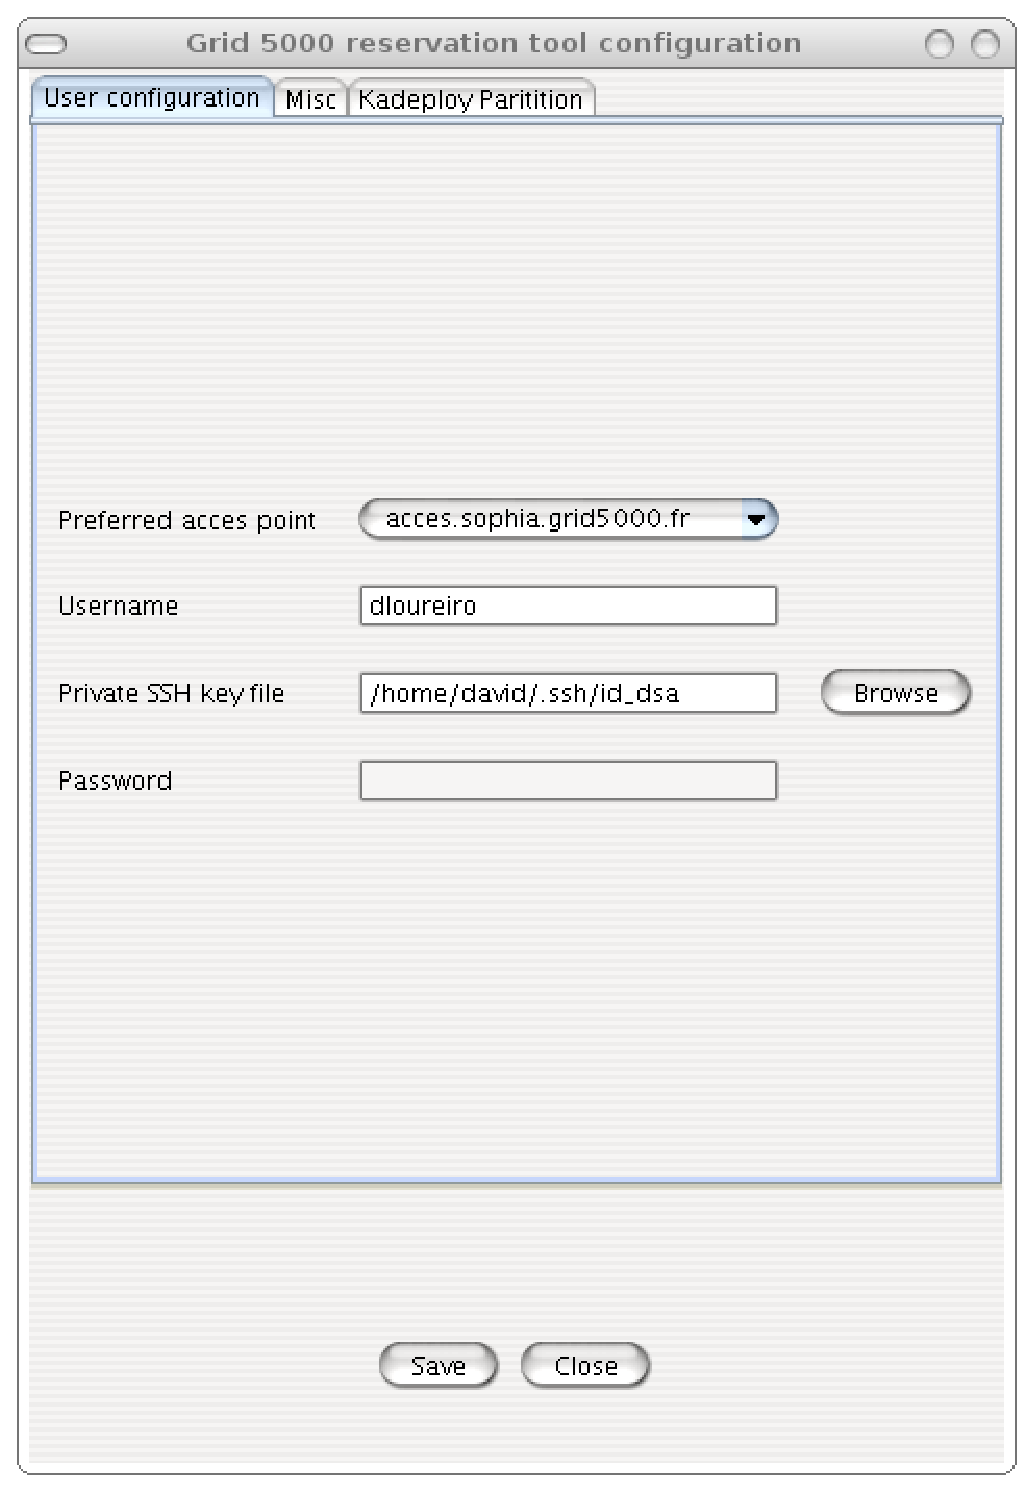
\includegraphics[width=0.4\linewidth]{figures/GRUDU_conf1.eps}
\caption{Configuration window: First tab}
\label{fig:cfg_tab1}
\end{figure}

The second configuration tab shown in figure~\ref{fig:cfg_tab2} allows the user
to configure the following parameters:
\begin{itemize}
  \item Enabling/Disabling a site: by default all sites are disabled.
  \item KaDeploy partition for each site (the same partition will be used for
  every clusters of that site).
  \item OAR batch Scheduler main version (you can choose between oar1 and oar2)
\end{itemize}

\begin{figure}[H]
\centering
\includegraphics[width=0.4\linewidth]{figures/GRUDU_conf2.eps}
\caption{Configuration window: Second tab}
\label{fig:cfg_tab2}
\end{figure}

The third tar shown in figure~\ref{fig:cfg_tab3} allows the user to configure
the KaDeploy partition for every clusters independently.

\begin{figure}[H]
\centering
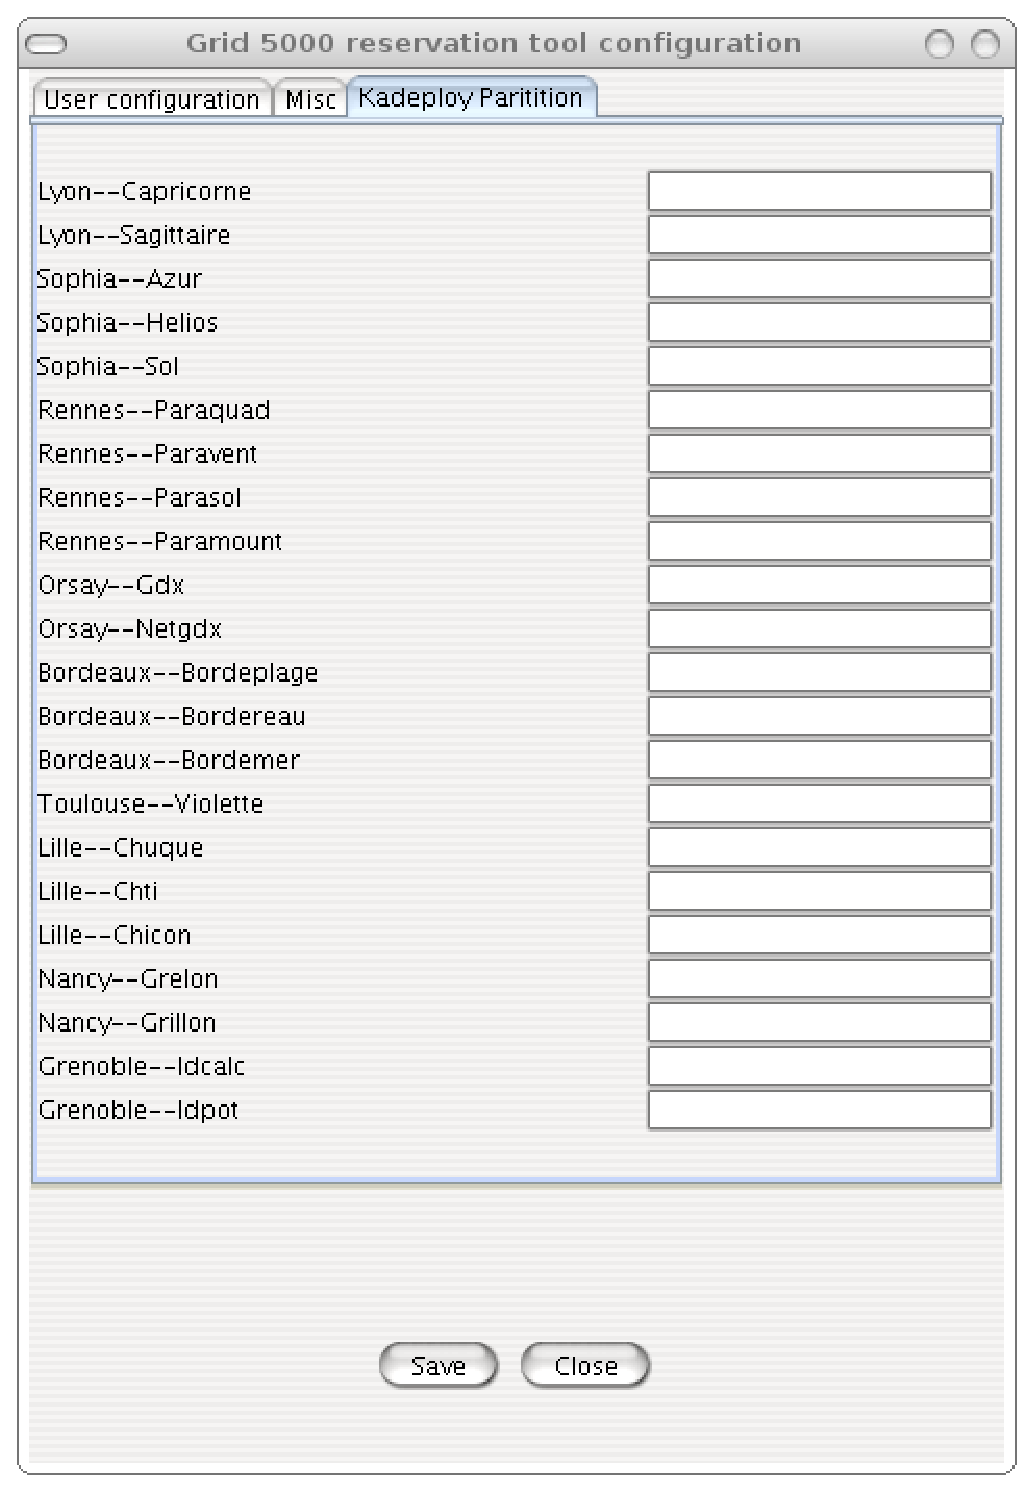
\includegraphics[width=0.4\linewidth]{figures/GRUDU_conf3.eps}
\caption{Configuration window: Third tab}
\label{fig:cfg_tab3}
\end{figure}

%******************************************%

% inclusion de GUM_interface.tex
%****************************************************************************%
%* Interface Presentation                                                   *%
%*                                                                          *%
%* Author(s):                                                               *%
%* - Abdelkader AMAR (Abdelkader.Amar@ens-lyon.fr)                          *%
%* - David LOUREIRO (David.Loureiro@ens-lyon.fr)                            *%
%*                                                                          *%
%* $LICENSE$                                                                *%
%****************************************************************************%
%* $Id: GUM_interface.tex,v 1.4 2007/11/29 16:03:21 dloureir Exp $
%* $Log: GUM_interface.tex,v $
%* Revision 1.4  2007/11/29 16:03:21  dloureir
%* typo corrections
%*
%* Revision 1.3  2007/11/08 16:28:53  dloureir
%* Adding some corrections and updates
%*
%* Revision 1.2  2007/11/08 11:31:14  dloureir
%* Correcting the headers
%*
%****************************************************************************%

\chapter{Interface presentation}

\grudu is composed of one principal frame shown in Figure \ref{fig:GRUDU_main}.
From this frame the user will be able to:
\begin{itemize}
  \item Log in \gfk
  \item Monitor \gfk and his/her reservations
  \item Have a terminal on the preferred access frontale, the different sites,
  and the main node of each of his/her reservations on \gfk
  \item Deploy images through KaDeploy on the appropriate nodes
  \item Exchange files between the locale machine and \gfk but also synchronize
  files between \gfk frontends.
  \item Log out
  \item Display the Help of \grudu
\end{itemize}

\begin{figure}[H]
\centering
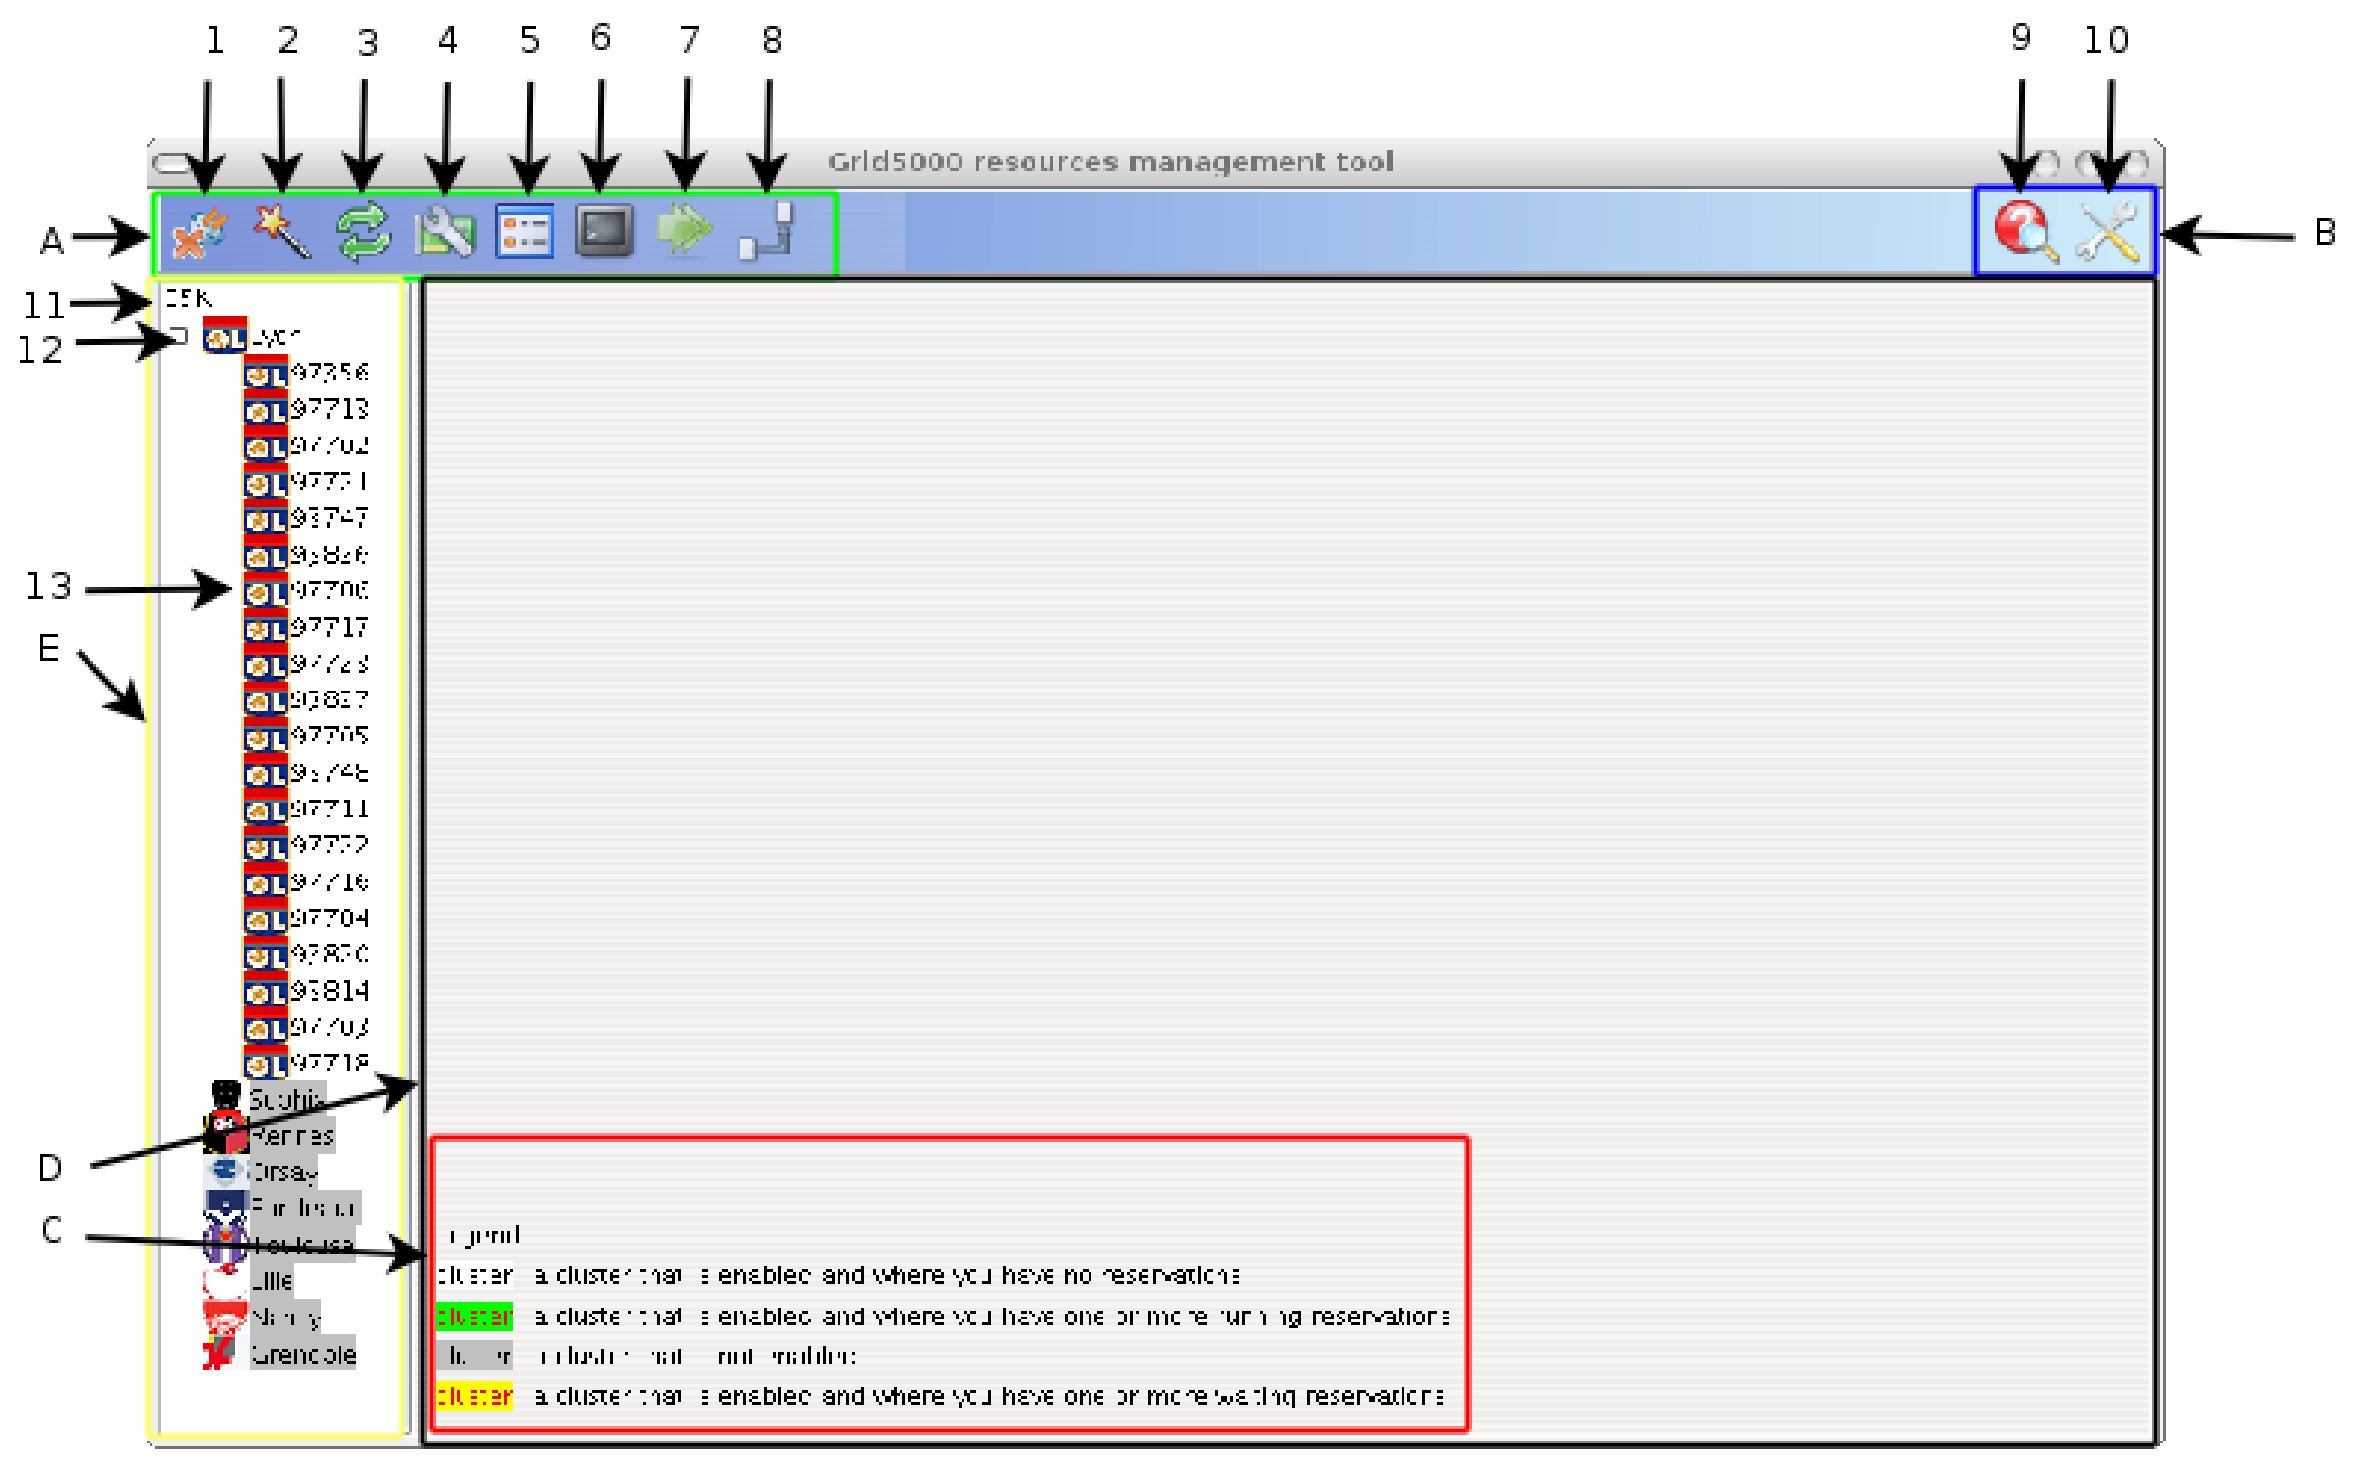
\includegraphics[width=\linewidth]{figures/GRUDU_interface_schema.eps}
\caption{Main interface of \grudu}
\label{fig:GRUDU_main}
\end{figure}

Legend of Figure \ref{fig:GRUDU_main}:
\begin{itemize}
  \item[A] Options toolbar (left-hand side).
  \begin{itemize}
    \item[1] Button used to log in \gfk (When connected to \gfk you will have a
    button to log out).
    \item[2] Button used to display the reservation frame.
    \item[3] Button used to update the \gfk tree of sites and jobs.
    \item[4] Button used to display the configuration frame.
    \item[5] Button used to display a summary of the information about \gfk and
    your reservations.
    \item[6] Button used to display a terminal on the preferred access point you
    have defined.
    \item[7] Button used to display the KaDeploy frame for the deployment of
    images with user-defined environments.
    \item[8] Button used to display the JFTP module for GRUDU. This module
    allows the user to transfert data between your locale machine and \gfk. You
    can also transfert data between the \gfk frontales.
  \end{itemize}
  \item[B] Options toolbar (right-hand side)
  \begin{itemize}
    \item[9] JavaHelp dedicated to the Help of GRUDU.
    \item[10] Application settings of GRUDU.
  \end{itemize}
  \item[C] Legend of the colors used for the sites, and jobs.
  \item[D] Main panel where information are displayed. Information about \gfk,
  the different sites and the jobs are displayed here.\item[]
  \item[E] \gfk sites and jobs.
  \begin{itemize}
    \item[11] Root node of the \gfk sites and jobs tree. This node
    allows you to display information about the grid. When right-clicking on this
    node, you can either update the \gfk view, open a shell on your preferred
    access point or delete all your reservations on \gfk.
    \item[12] Node corresponding to a site. Information about the site,
    i.e. the occupation of the nodes and the existing reservations on this
    site. When right-clicking on a site node, you can either delete the
    reservations you have on the site or open a shell on the site frontale.
    \item[13] Node corresponding to a job. Information on the job are displayed
    in the information panel. When right-clicking on that node, you will able to
    delete the corresponding reservation, update the site view or open a shell on
    the main node of the corresponding job.
  \end{itemize}  
\end{itemize}

A tip of the day frame is shown (if you want so) at GRUDU startup and presents
you some tips for the use of GRUDU. You can enable/disable the frame in the
application configuration frame (see \ref{chapter:application_settings}).

\begin{figure}[H]
\centering
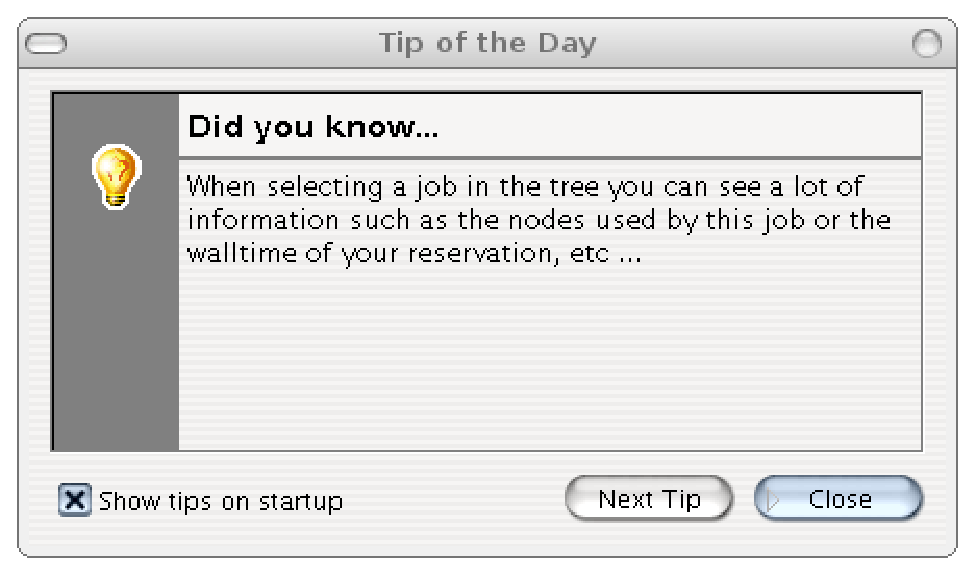
\includegraphics[width=0.6\linewidth]{figures/GRUDU_totd.eps}
\caption{Tip of the day for GRUDU}
\label{fig:GRUDU_totd}
\end{figure}

%******************************************%

% inclusion de GUM_resources.tex
%****************************************************************************%
%* Resources allocation                                                     *%
%*                                                                          *%
%* Author(s):                                                               *%
%* - Abdelkader AMAR (Abdelkader.Amar@ens-lyon.fr)                          *%
%* - David LOUREIRO (David.Loureiro@ens-lyon.fr)                            *%
%*                                                                          *%
%* $LICENSE$                                                                *%
%****************************************************************************%
%* $Id: GUM_resources.tex,v 1.4 2007/11/29 16:03:21 dloureir Exp $
%* $Log: GUM_resources.tex,v $
%* Revision 1.4  2007/11/29 16:03:21  dloureir
%* typo corrections
%*
%* Revision 1.3  2007/11/08 16:28:54  dloureir
%* Adding some corrections and updates
%*
%* Revision 1.2  2007/11/08 11:31:14  dloureir
%* Correcting the headers
%*
%****************************************************************************%
\chapter{Resources allocation}

\section{Using OAR interface}
\label{sec:oar}

The most used operation is probably the resources allocation. In \gfk,
this operation can be done by the OAR system. \grudu provides an easy way
to manipulate OAR (either the OAR1 or OAR2 versions). The resources allocation window on
Figure \ref{fig:cfg_tab1} shows a map of France with \gfk sites~\footnote{You
can allocate resources only on enabled sites} and jobs characteristics (time,
queue, oargridsub behaviour, the script to launch). 

These information are presented on the first tab of the
window. The second tab provides the definition of the properties for the
different sites.

Since some sites include more than one cluster, you have to click first on the
site, and then select the number of desired nodes for each cluster or you can
specify that you do not care where they are located).
When selecting resources numbers, the map displays the total number of requested
resources for each site\footnote{When the mouse is over the site box, a tooltip
will tell you the repartition of the nodes you may want to reserve}. Jobs characteristics
are:
\begin{itemize}
  \item Time parameters: date and reservation walltime. The starting time can
  be specified manually, or through the use of a calendar for the day and
  through boxes where you can specify the hour, the minute and the second. For
  the walltime you have to define the number of hours and the minutes of your reservation.
  \item Queue: default, deploy (for KaDeploy) or \textit{allow\_classic\_ssh}
  \footnote{specific for OAR2 but corresponds to default for OAR1}.
  \item OARGridSub behaviour: the user can specify if the reservation should be
  done with the OARGridSub behaviour, i.e. when the user chooses to realize
  several reservations on different sites, if one fails, all the previous
  successful reservations are deleted.
  \item A script to launch: The user can specify a script that will be launched
  in order to be executed on the reserved nodes. The reservation will be stopped
  when the script ends.
\end{itemize}

\begin{figure}[H]
\centering
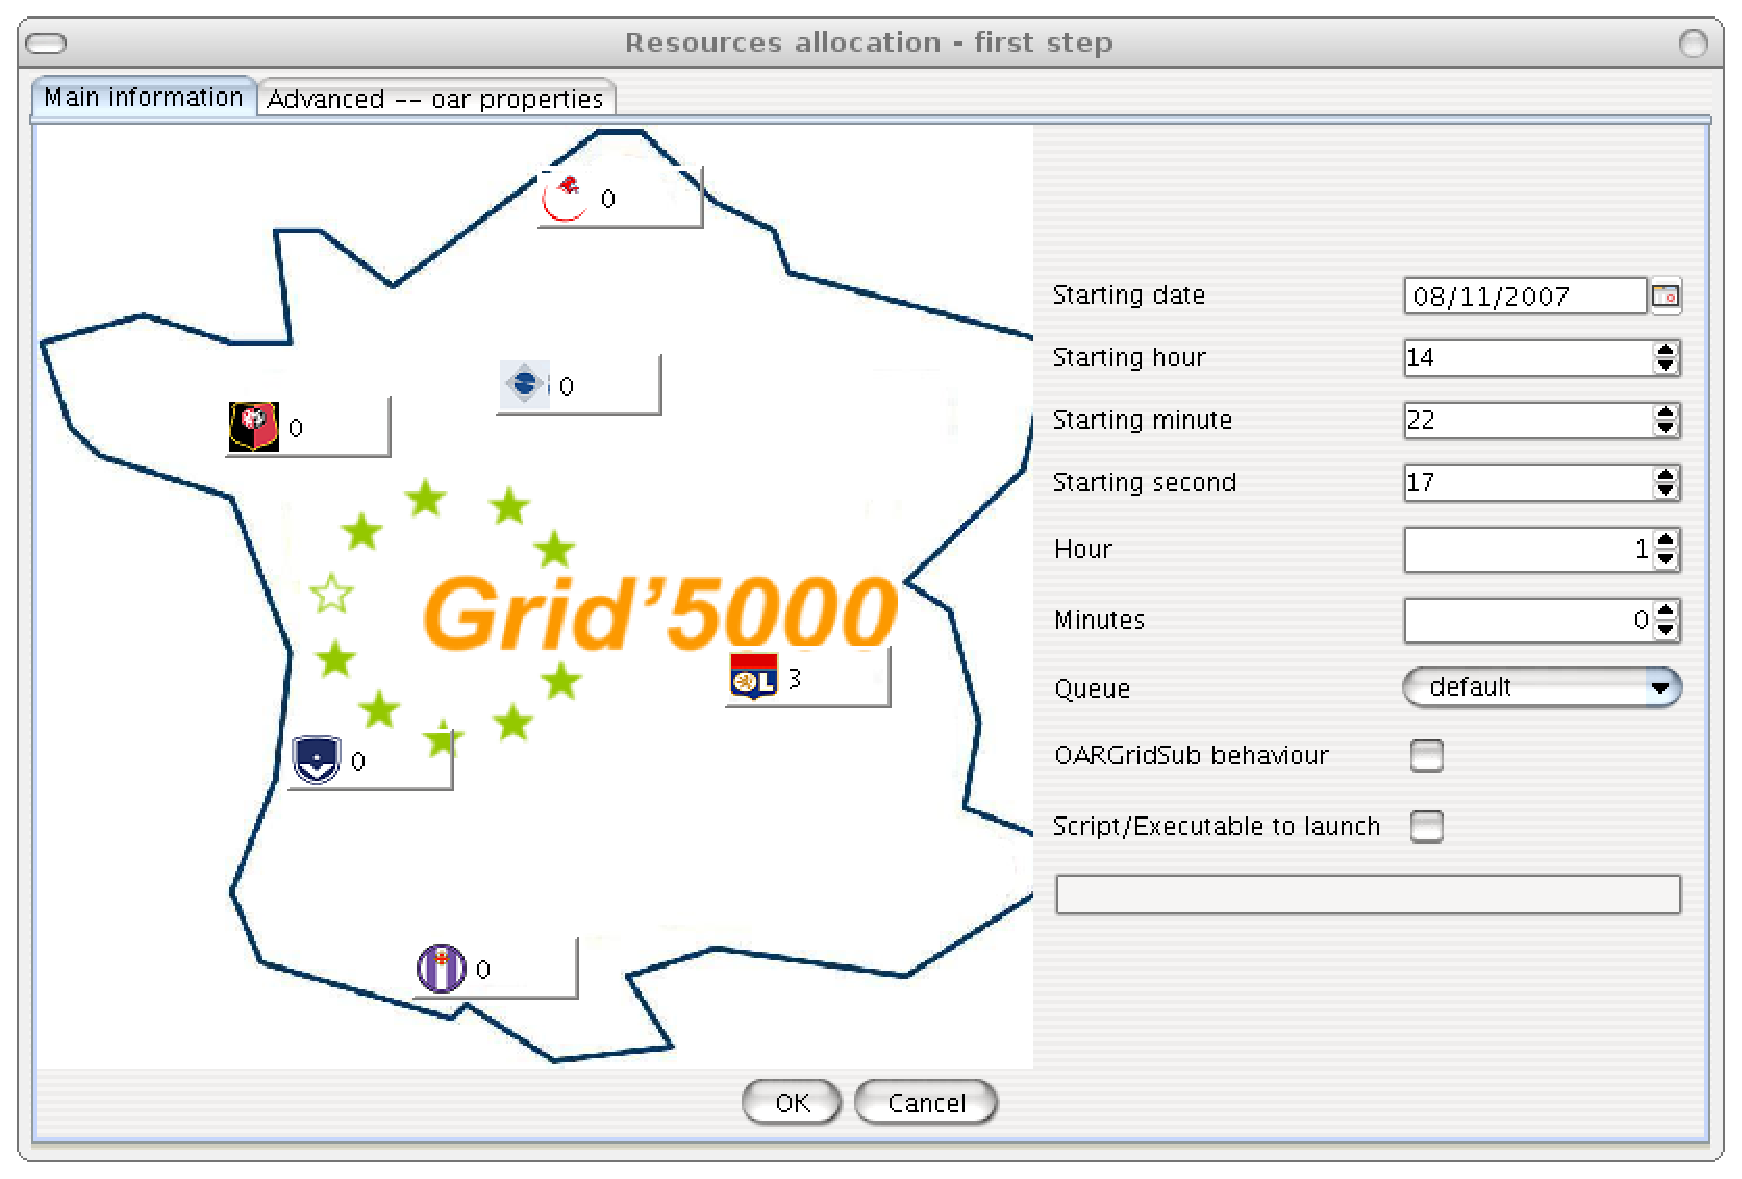
\includegraphics[width=0.6\linewidth]{figures/GRUDU_allocation_1.eps}
\caption{Resources allocation frame -- Main panel}
\label{fig:cfg_allocation1}
\end{figure}

Concerning the second tab of the window presented on Figure \ref{fig:cfg_tab2},
it allows the user to define the OAR properties that will be used for
 the reservation.
 
\begin{figure}[H]
\centering
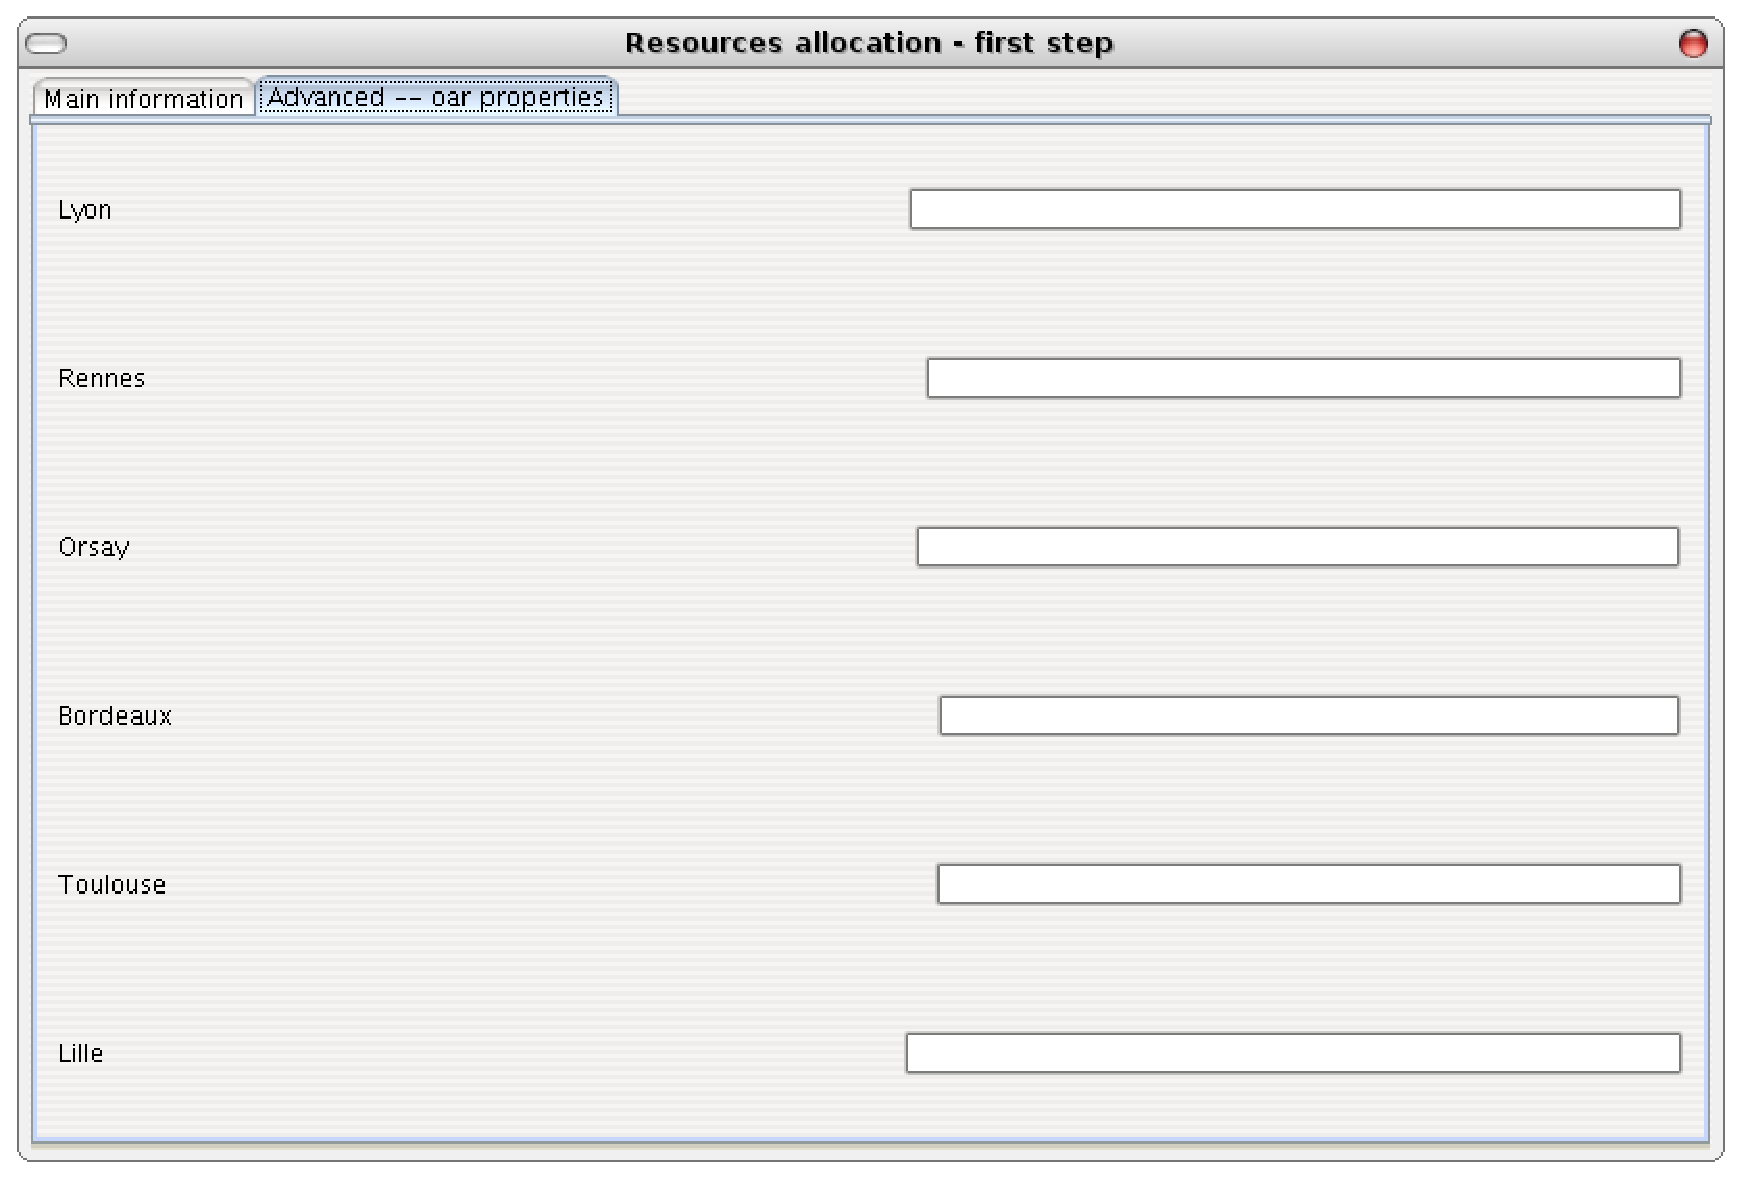
\includegraphics[width=0.6\linewidth]{figures/GRUDU_allocation_2.eps}
\caption{Resources allocation frame -- OAR properties for the reservation}
\label{fig:cfg_allocation2}
\end{figure}

After the reservation, a status frame summarizes the information about the
success (or not) of your jobs submission.

\begin{figure}[H]
\centering

\includegraphics[width=0.6\linewidth]{figures/GRUDU_reservation1.eps}
\caption{Resources allocation frame -- Reservation status}
\label{fig:reservation_status}
\end{figure}

%******************************************%

% inclusion de GUM_monitoring.tex
%****************************************************************************%
%* Monitoring Grid'5000                                                     *%
%*                                                                          *%
%* Author(s):                                                               *%
%* - Abdelkader AMAR (Abdelkader.Amar@ens-lyon.fr)                          *%
%* - David LOUREIRO (David.Loureiro@ens-lyon.fr)                            *%
%*                                                                          *%
%* $LICENSE$                                                                *%
%****************************************************************************%
%* $Id: GUM_monitoring.tex,v 1.6 2007/11/29 16:03:21 dloureir Exp $
%* $Log: GUM_monitoring.tex,v $
%* Revision 1.6  2007/11/29 16:03:21  dloureir
%* typo corrections
%*
%* Revision 1.5  2007/11/29 10:49:02  dloureir
%* correcting the wrong reference
%*
%* Revision 1.4  2007/11/08 16:53:48  dloureir
%* Adding the ganglia part in the User's Manual
%*
%* Revision 1.3  2007/11/08 16:28:54  dloureir
%* Adding some corrections and updates
%*
%* Revision 1.2  2007/11/08 11:31:14  dloureir
%* Correcting the headers
%*
%****************************************************************************%
\chapter{Monitoring \gfk}
To monitor \gfk, three views can be displayed:
\begin{itemize}
  \item The first view in Figure \ref{fig:GRUDU_view_g5k} corresponds to the
  \gfk view. You can see the state of the grid in term of
  free/occupied/dead/absent/suspected/possessed nodes for each site and for
  the entire grid.
  Added to the states of the nodes, you can also see which nodes you have reserved.
  You can also see a table summarizing these information. Finally you have a
  table of your reservation(s) on the grid. Thanks to two buttons you can save your
  reservation(s) in a directory for a future use (for example in the DIET Mapping
  Tool or with the XMLGoDIETGenerator)
  \begin{figure}[H]
	\centering
	\includegraphics[width=0.5\linewidth]{figures/GRUDU_interface2.eps}
	\caption{Grid'5000 view}
	\label{fig:GRUDU_view_g5k}
  \end{figure}
  \item The second view in Figure \ref{fig:GRUDU_view_site} corresponds to a
  site view. A graph represents the different numbers of nodes for each different
  state ant the ones corresponding to your possible reservation(s). A table 
  presents these information in a different way. Another table displays the 
  reservation(s) realized on the site. You can also display a Gantt chart of the 
  different reservations of the cluster to know when you are able to reserve.
  
  If you selected the Ganglia plugin at the installation step, you also have a
  button bar on the right hand side of the frame that will be populated with a
  Ganglia information button allowing you to get low-level information on every
  machines of the site (data are instantaneous).
	\begin{figure}[H]
  \centering 
  \begin{tabular}{cc}
  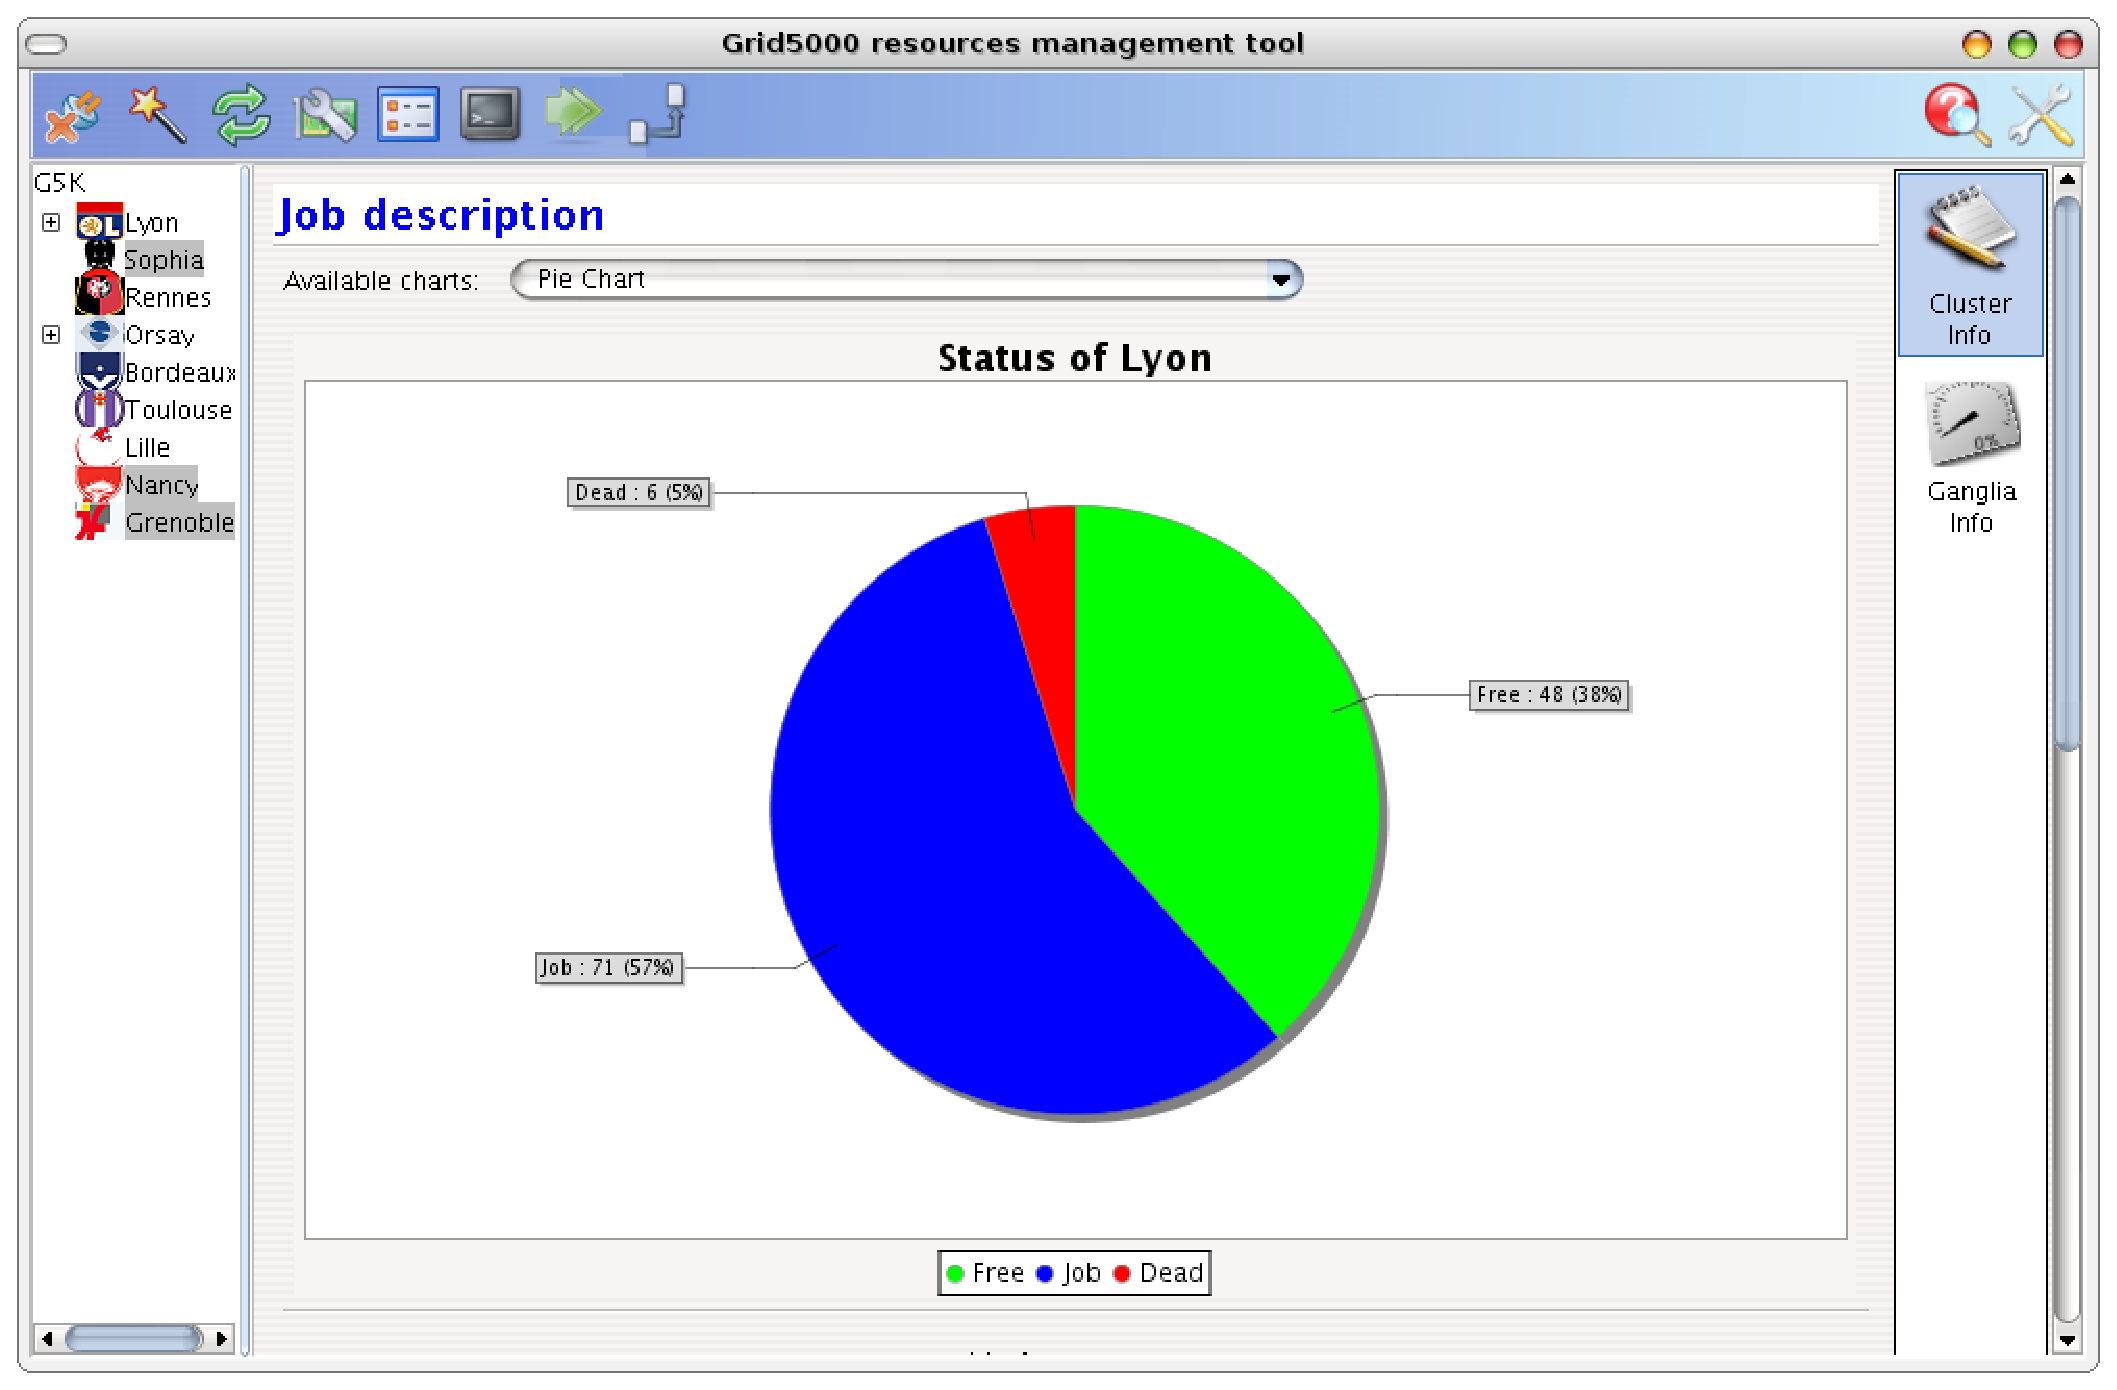
\includegraphics[width=0.5\linewidth]{figures/GRUDU_interface3.eps} &
  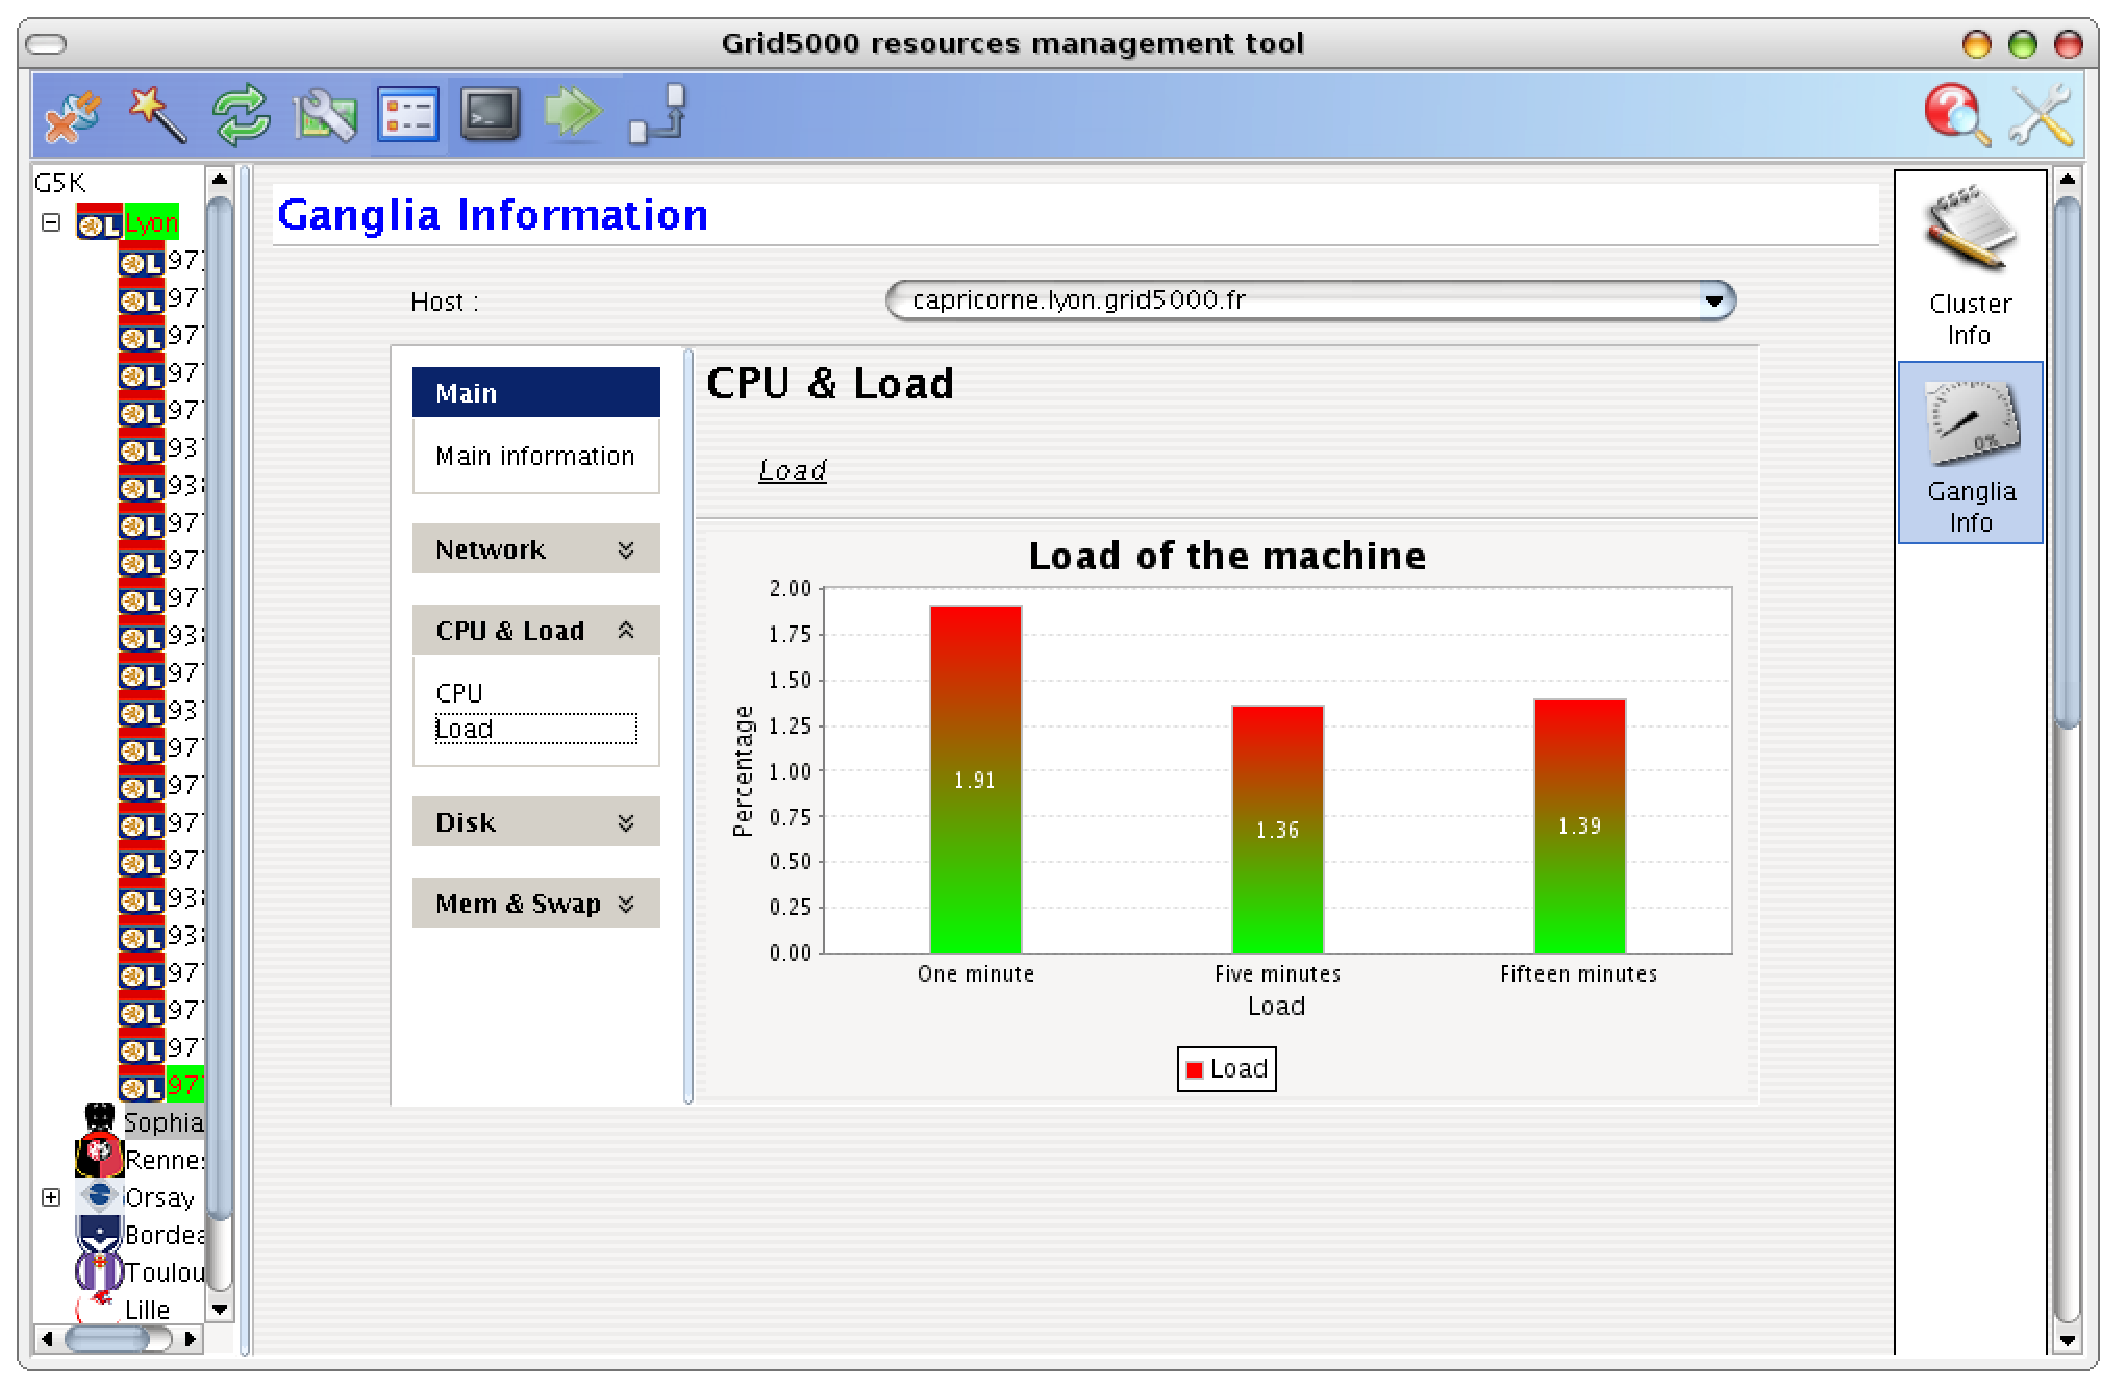
\includegraphics[width=0.5\linewidth]{figures/GRUDU_interface3_ganglia.eps}
  \end{tabular}
	\caption{Site view}
	\label{fig:GRUDU_view_site}
  \end{figure}
  \item  The third view in figure \ref{fig:GRUDU_view_job} corresponds to the
  job view. Here you can see the different information of the job such as the
  nodes of the reservation, the job state, the walltime, etc \ldots
  
  If you selected the Ganglia plugin at the installation step, you also have a
  button bar on the right hand side of the frame that will be populated with a
  Ganglia history information button allowing you to get an history on the
  low-level information concerning the nodes of your reservation. \begin{figure}[H]
  \centering
  \begin{tabular}{cc}
  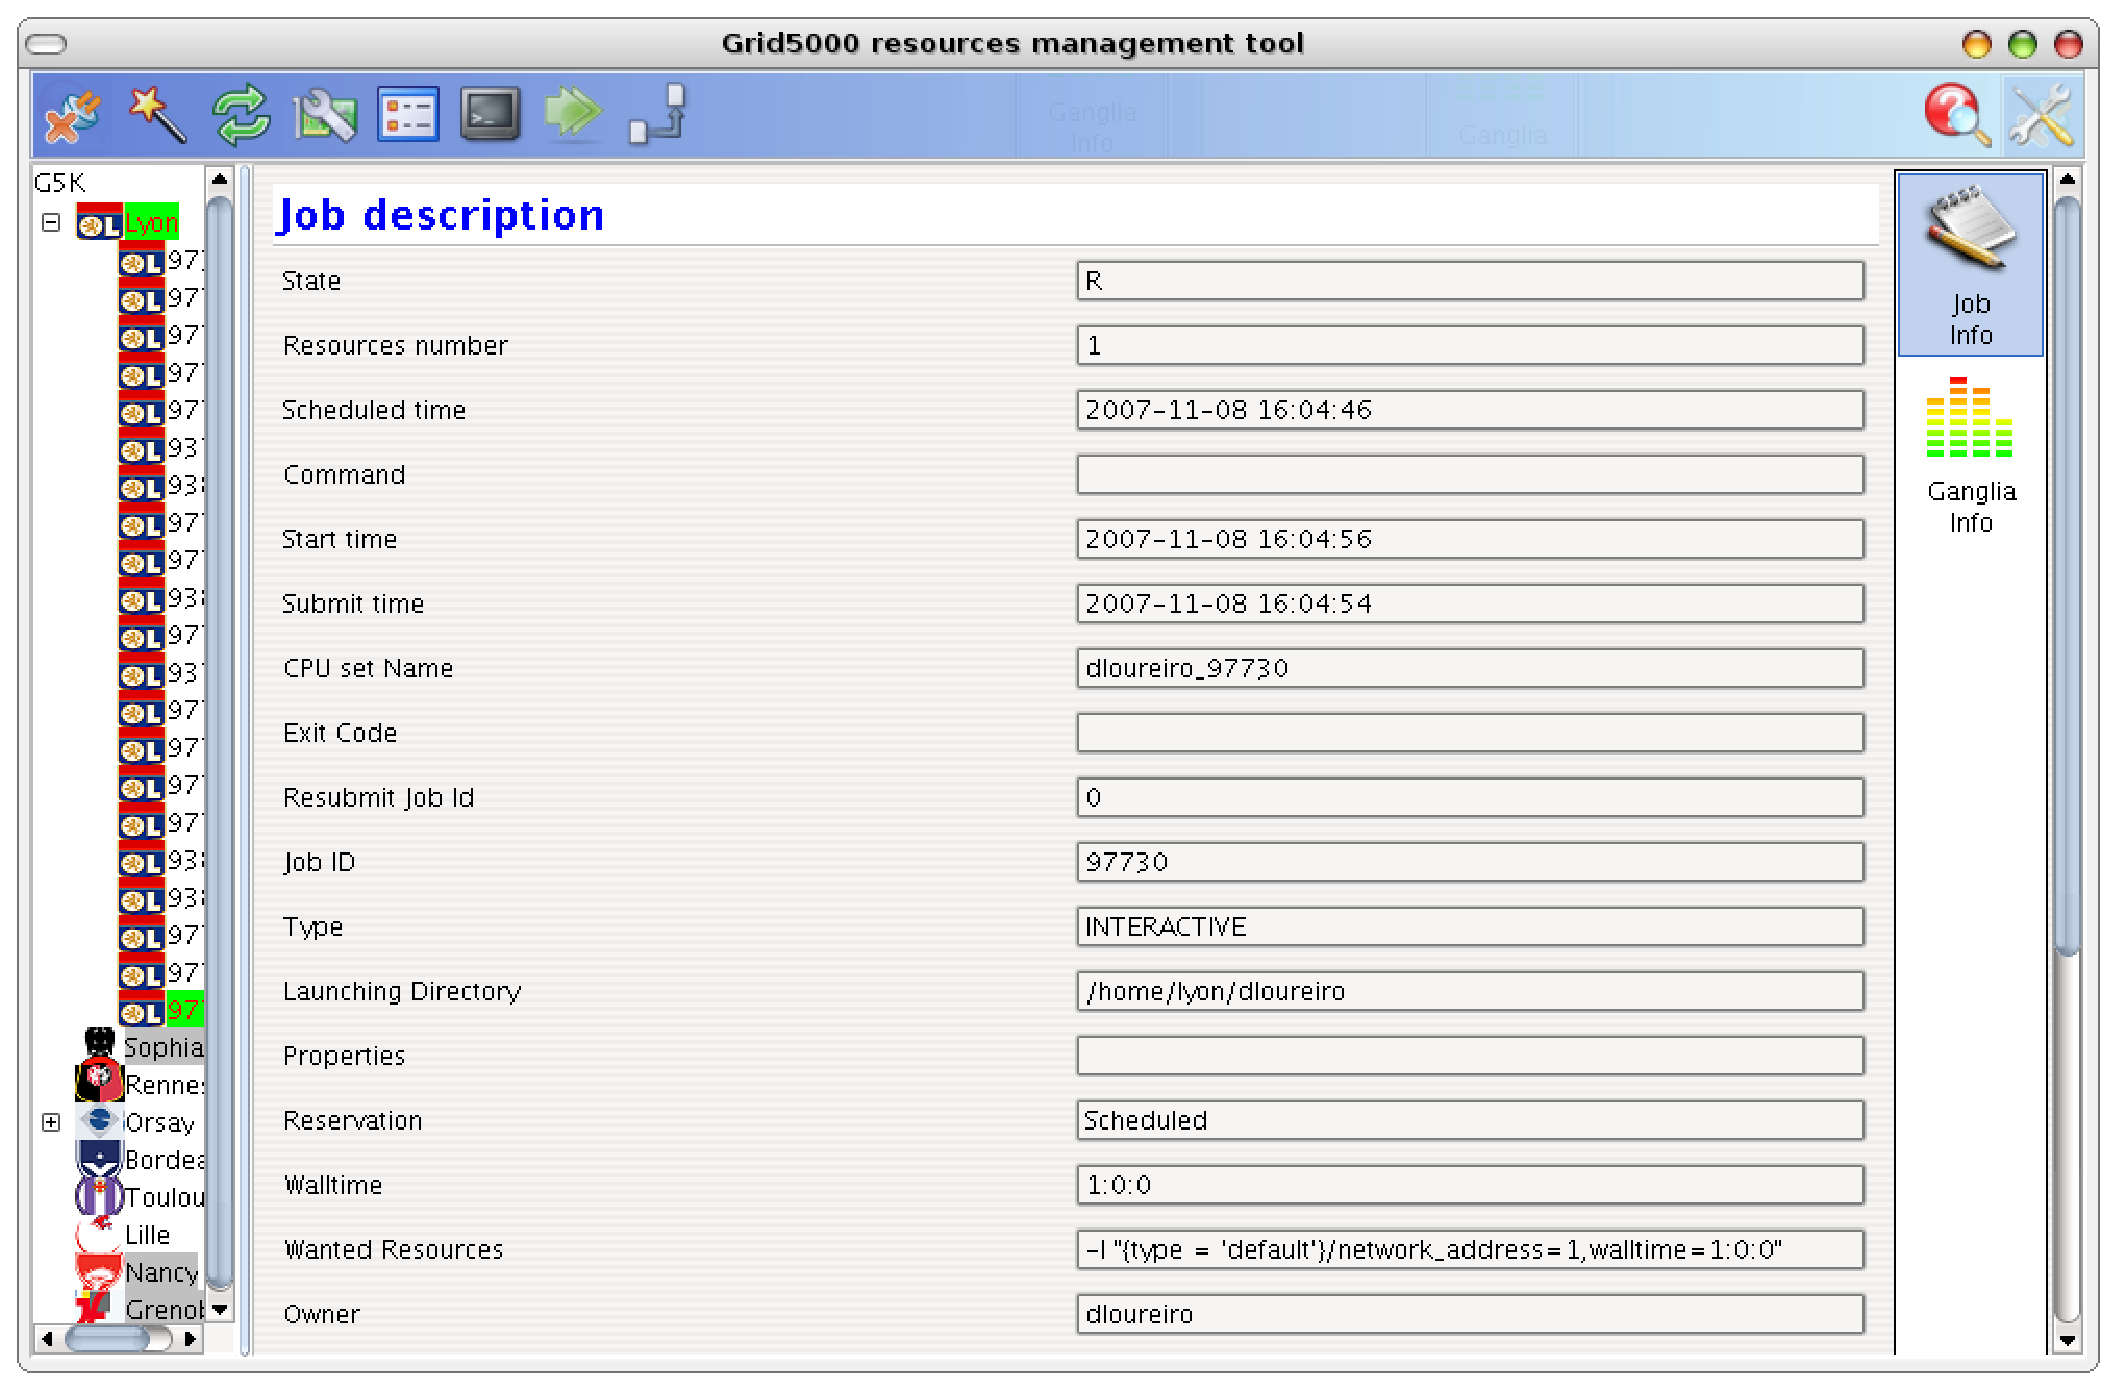
\includegraphics[width=0.5\linewidth]{figures/GRUDU_interface4.eps} &
  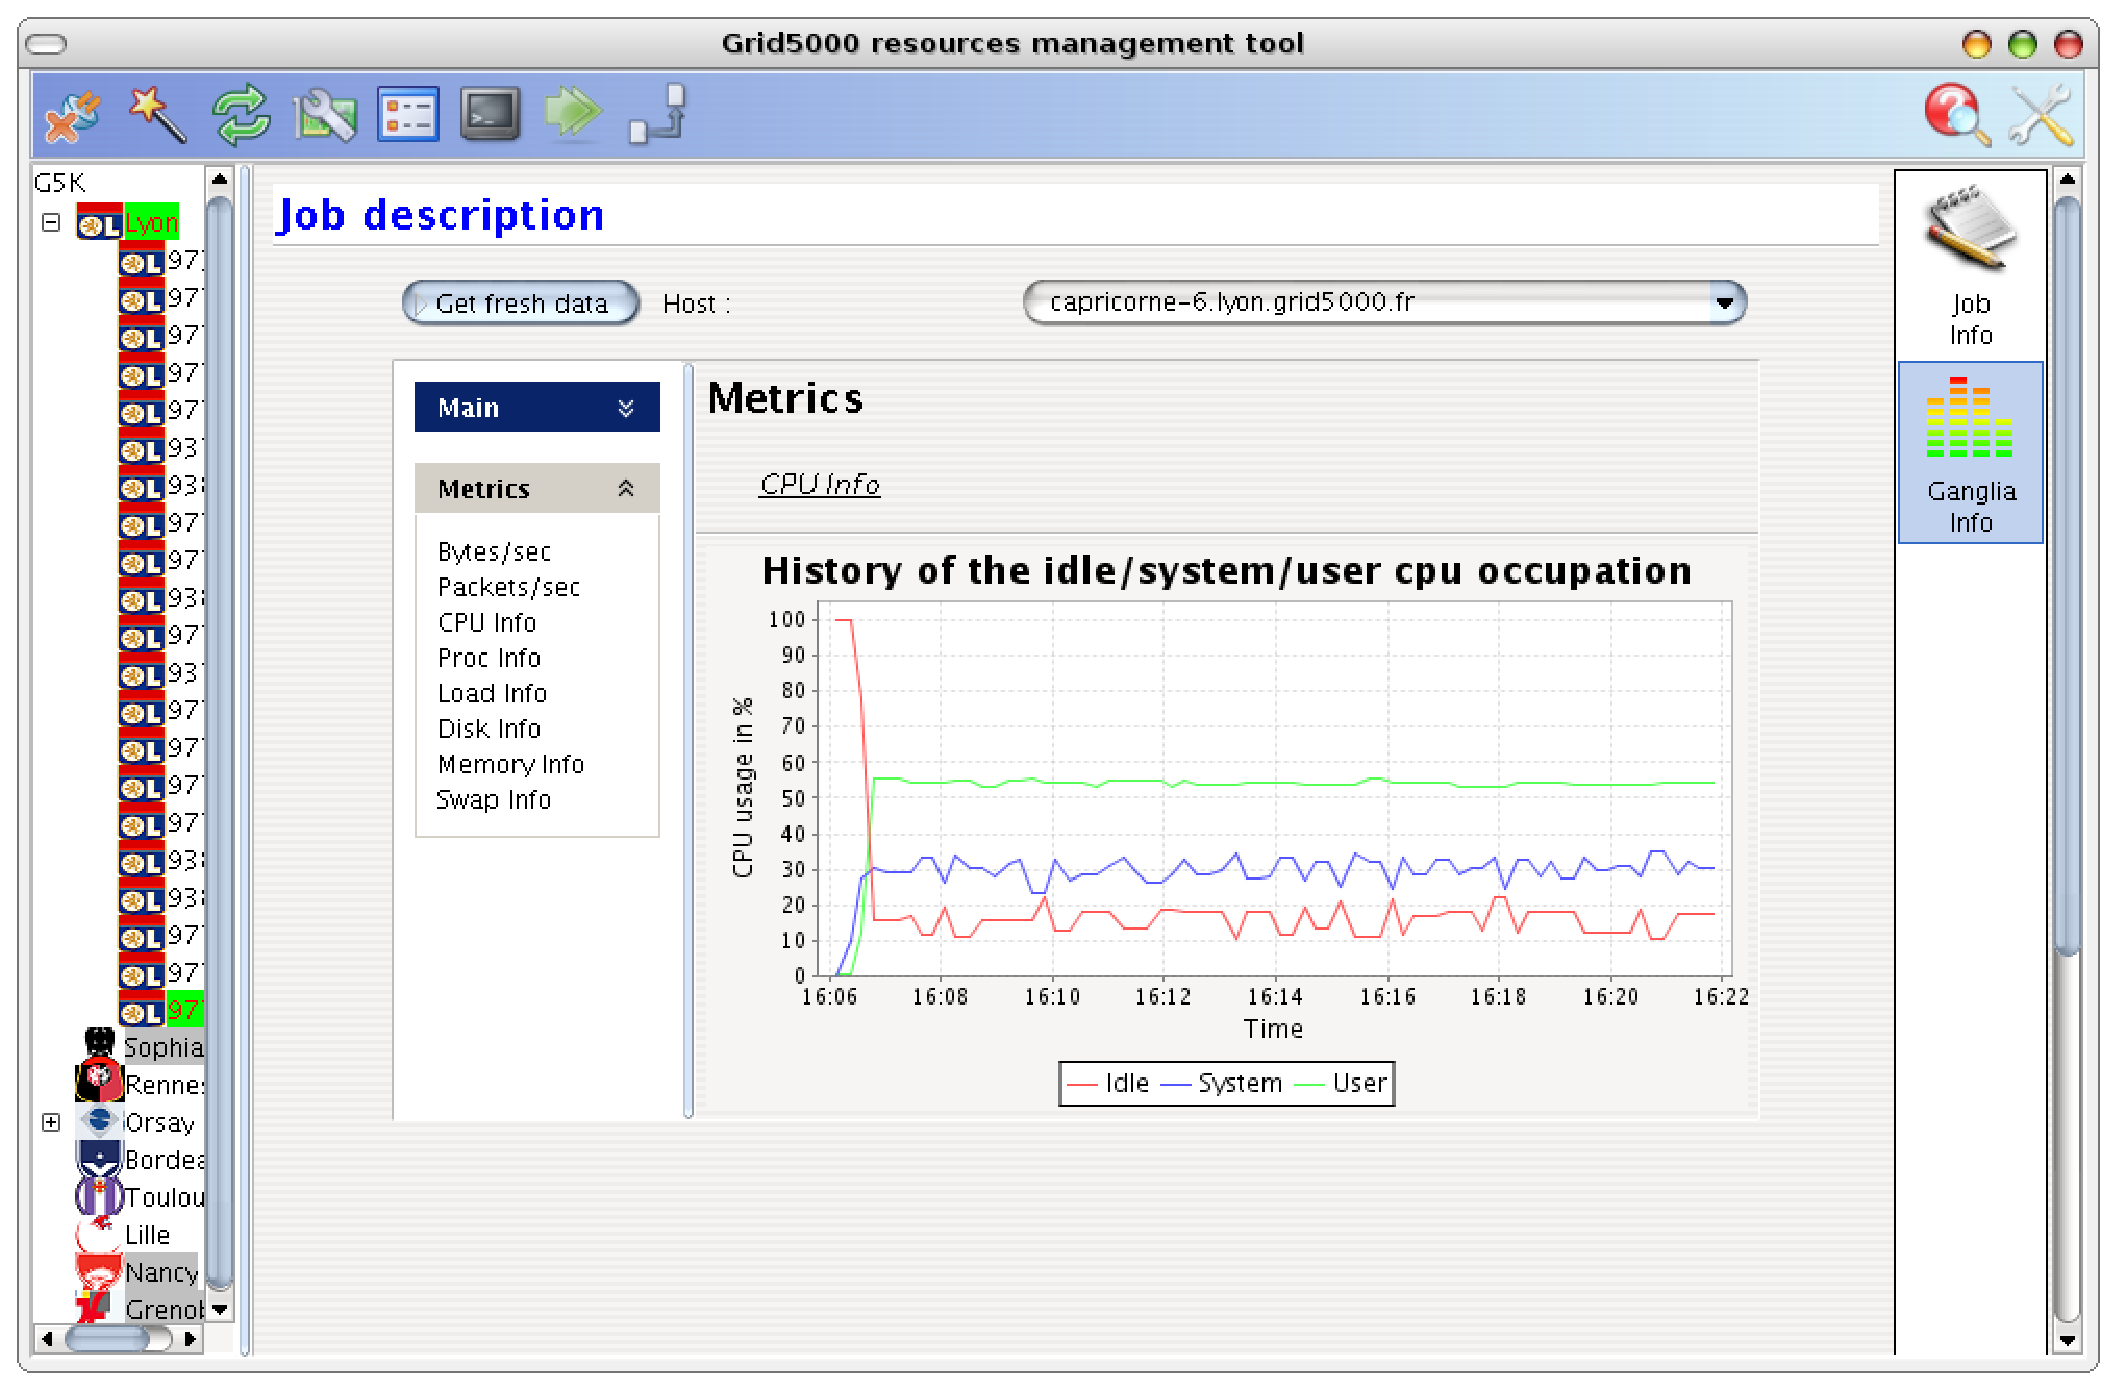
\includegraphics[width=0.5\linewidth]{figures/GRUDU_interface4_ganglia.eps}
  \end{tabular}
	\caption{Job view}
	\label{fig:GRUDU_view_job}
  \end{figure}
\end{itemize}

%******************************************%

%inclusion de GUM_Ganglia.tex
%****************************************************************************%
%* Ganglia Module                                                           *%
%*                                                                          *%
%* Author(s):                                                               *%
%* - Abdelkader AMAR (Abdelkader.Amar@ens-lyon.fr)                          *%
%* - David LOUREIRO (David.Loureiro@ens-lyon.fr)                            *%
%*                                                                          *%
%* $LICENSE$                                                                *%
%****************************************************************************%
%* $Id: GUM_Ganglia.tex,v 1.2 2007/11/29 16:03:21 dloureir Exp $
%* $Log: GUM_Ganglia.tex,v $
%* Revision 1.2  2007/11/29 16:03:21  dloureir
%* typo corrections
%*
%* Revision 1.1  2007/11/08 16:53:48  dloureir
%* Adding the ganglia part in the User's Manual
%*
%* Revision 1.2  2007/11/08 11:31:14  dloureir
%* Correcting the headers
%*
%****************************************************************************%
\chapter{The Ganglia module for \grudu}

\section{Ganglia short introduction}

Ganglia is a scalable distributed monitoring system for high-performance
computing systems such as clusters and Grids. It is based on a hierarchical
design targeted at federations of clusters. It leverages widely used
technologies such as XML for data representation, XDR for compact, portable
data transport, and RRDtool for data storage and visualization. It uses
carefully engineered data structures and algorithms to achieve very low
per-node overheads and high concurrency. The implementation is robust, has been
ported to an extensive set of operating systems and processor architectures,
and is currently in use on thousands of clusters around the world. It has been
used to link clusters across university campuses and around the world and can
scale to handle clusters with 2000 nodes.          

Ganglia is an open-source project that grew out of the University of
California, Berkeley Millennium Project which was initially funded in large
part by the National Partnership for Advanced Computational Infrastructure
(NPACI) and National Science Foundation RI Award EIA-9802069. NPACI is funded
by the National Science Foundation and strives to advance science by creating a
ubiquitous, continuous, and pervasive national computational infrastructure:
the Grid. Current support comes from Planet Lab: an open platform for
developing, deploying, and accessing planetary-scale services.       

You can find more information on the Ganglia Website at
\url{http://ganglia.sourceforge.net} 

\section{Ganglia plugin}

As Ganglia is installed on \gfk, the \grudu users can have access to the
information provided by the software inside \grudu.

If you selected the ganglia plugin during the installation step of \grudu, there
is two ways to use it:
\begin{itemize}
  \item From the site information panels, where you can have instantaneous
  low-level information about every nodes of the site (computation nodes but also
  frontends).
  \begin{figure}[H]
  \centering 
  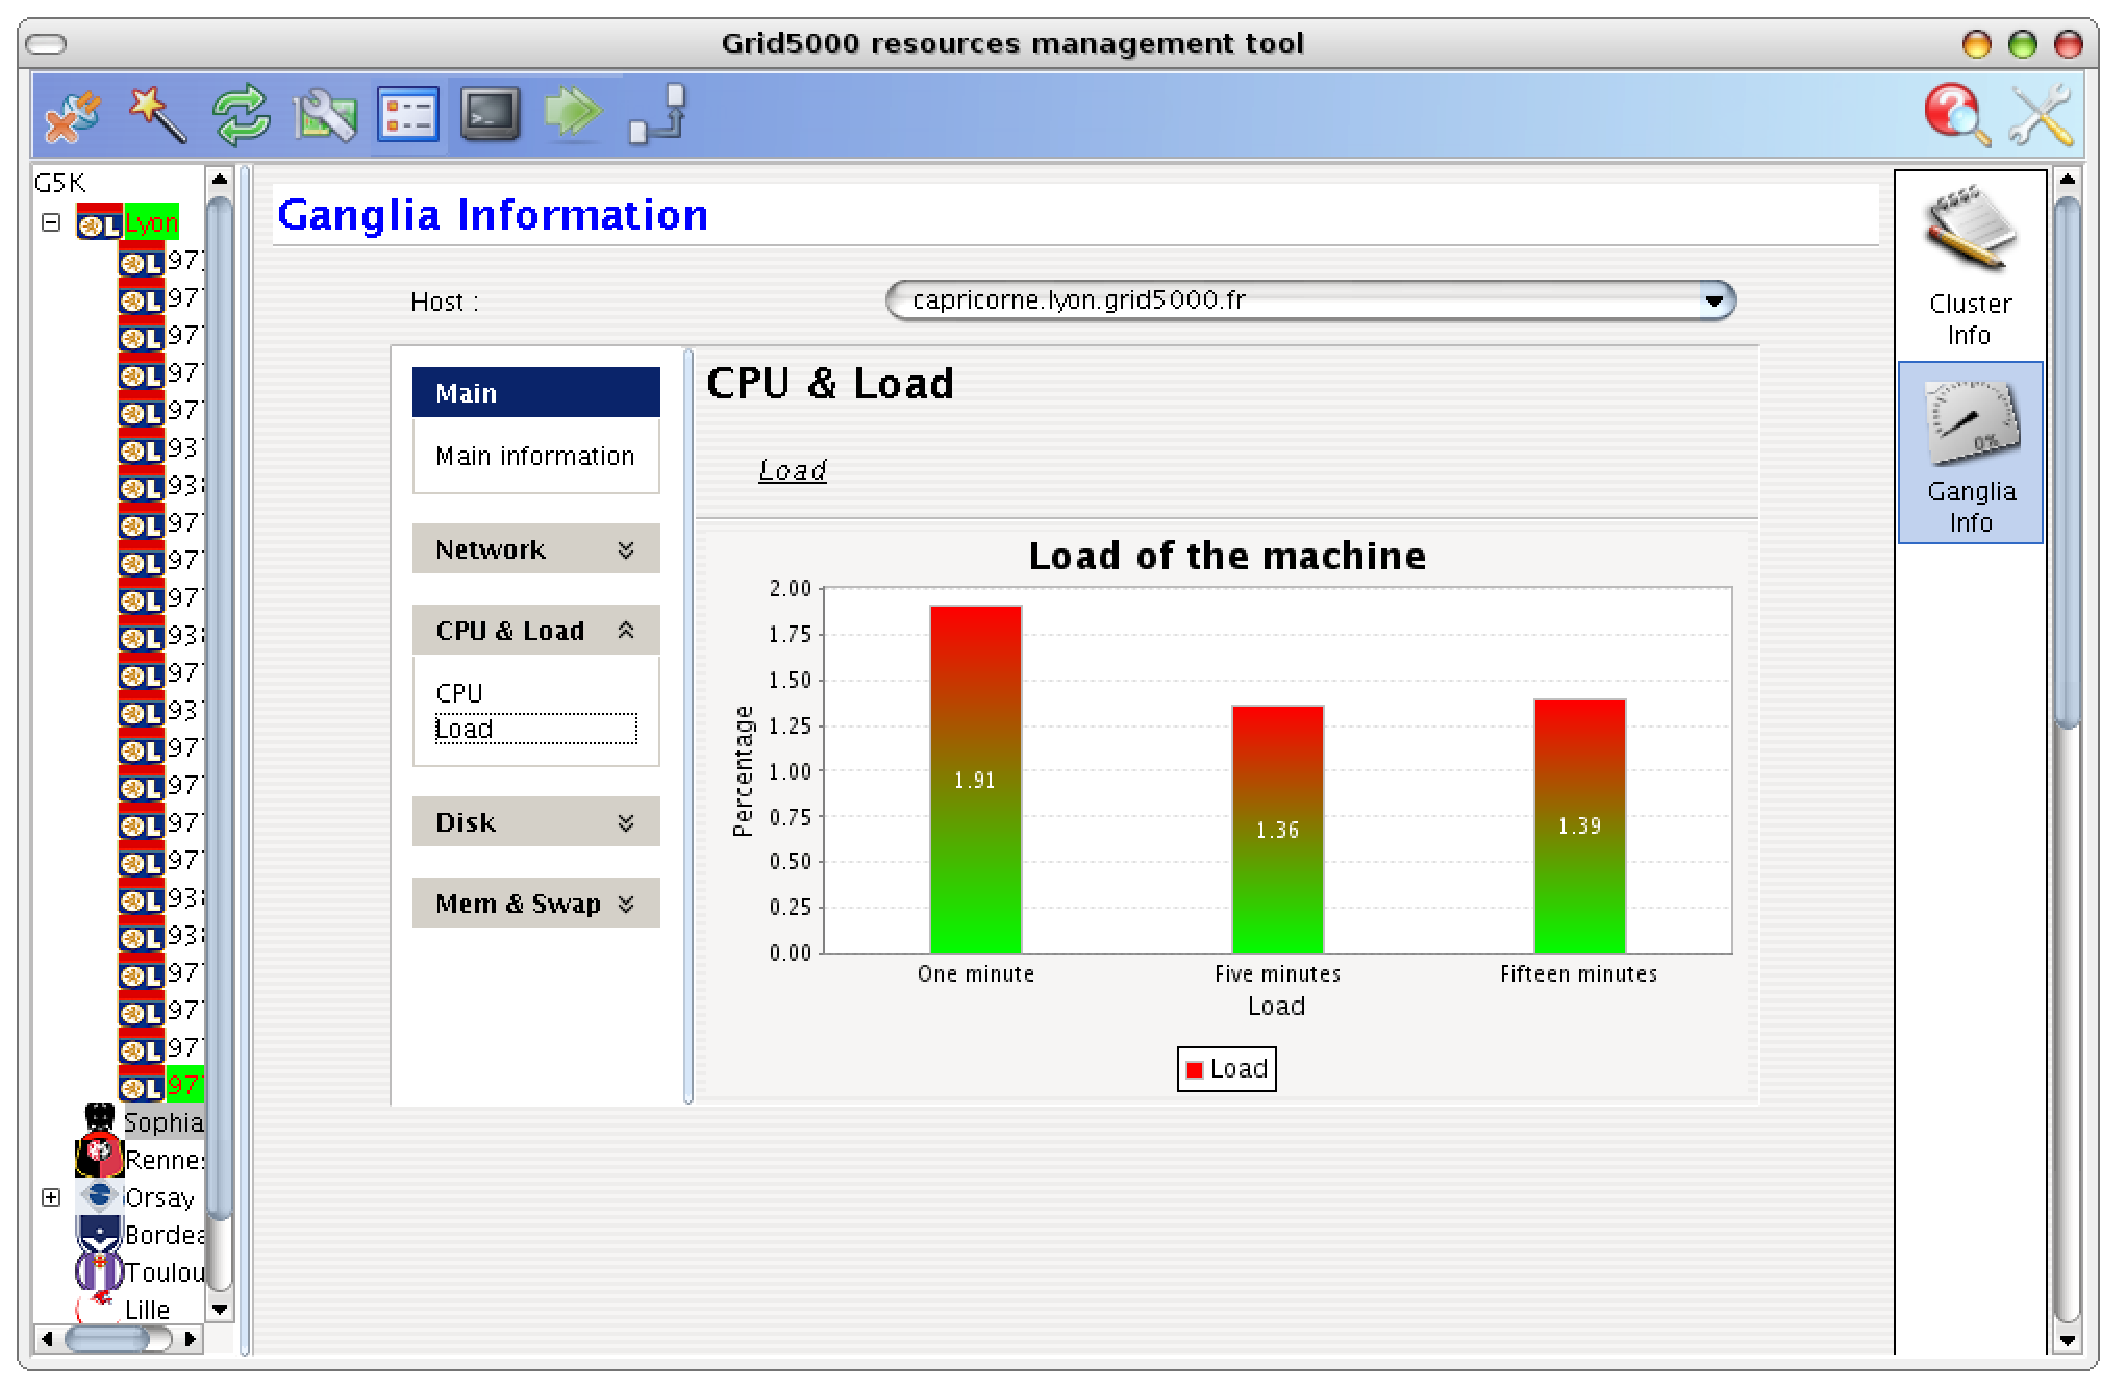
\includegraphics[width=0.5\linewidth]{figures/GRUDU_interface3_ganglia.eps}
	\caption{Ganglia plugin for the site view}
	\label{fig:GRUDU_view_site_ganglia}
  \end{figure}
  \item From the job information panels, where you can get the history of the
  low-level information brought to you by Ganglia. Concerning the generation of
  the history you have first to configure the history generation, which means defining:
  \begin{description}
  \item the period of data refreshing (of the form : hh:mm:ss)
  \item the range of the chart (same format)
  \item the path to the java home on the main node of your reservation for the
  launch of the remote jar creating the history.
  \end{description}
  \begin{figure}[H]
  \centering
  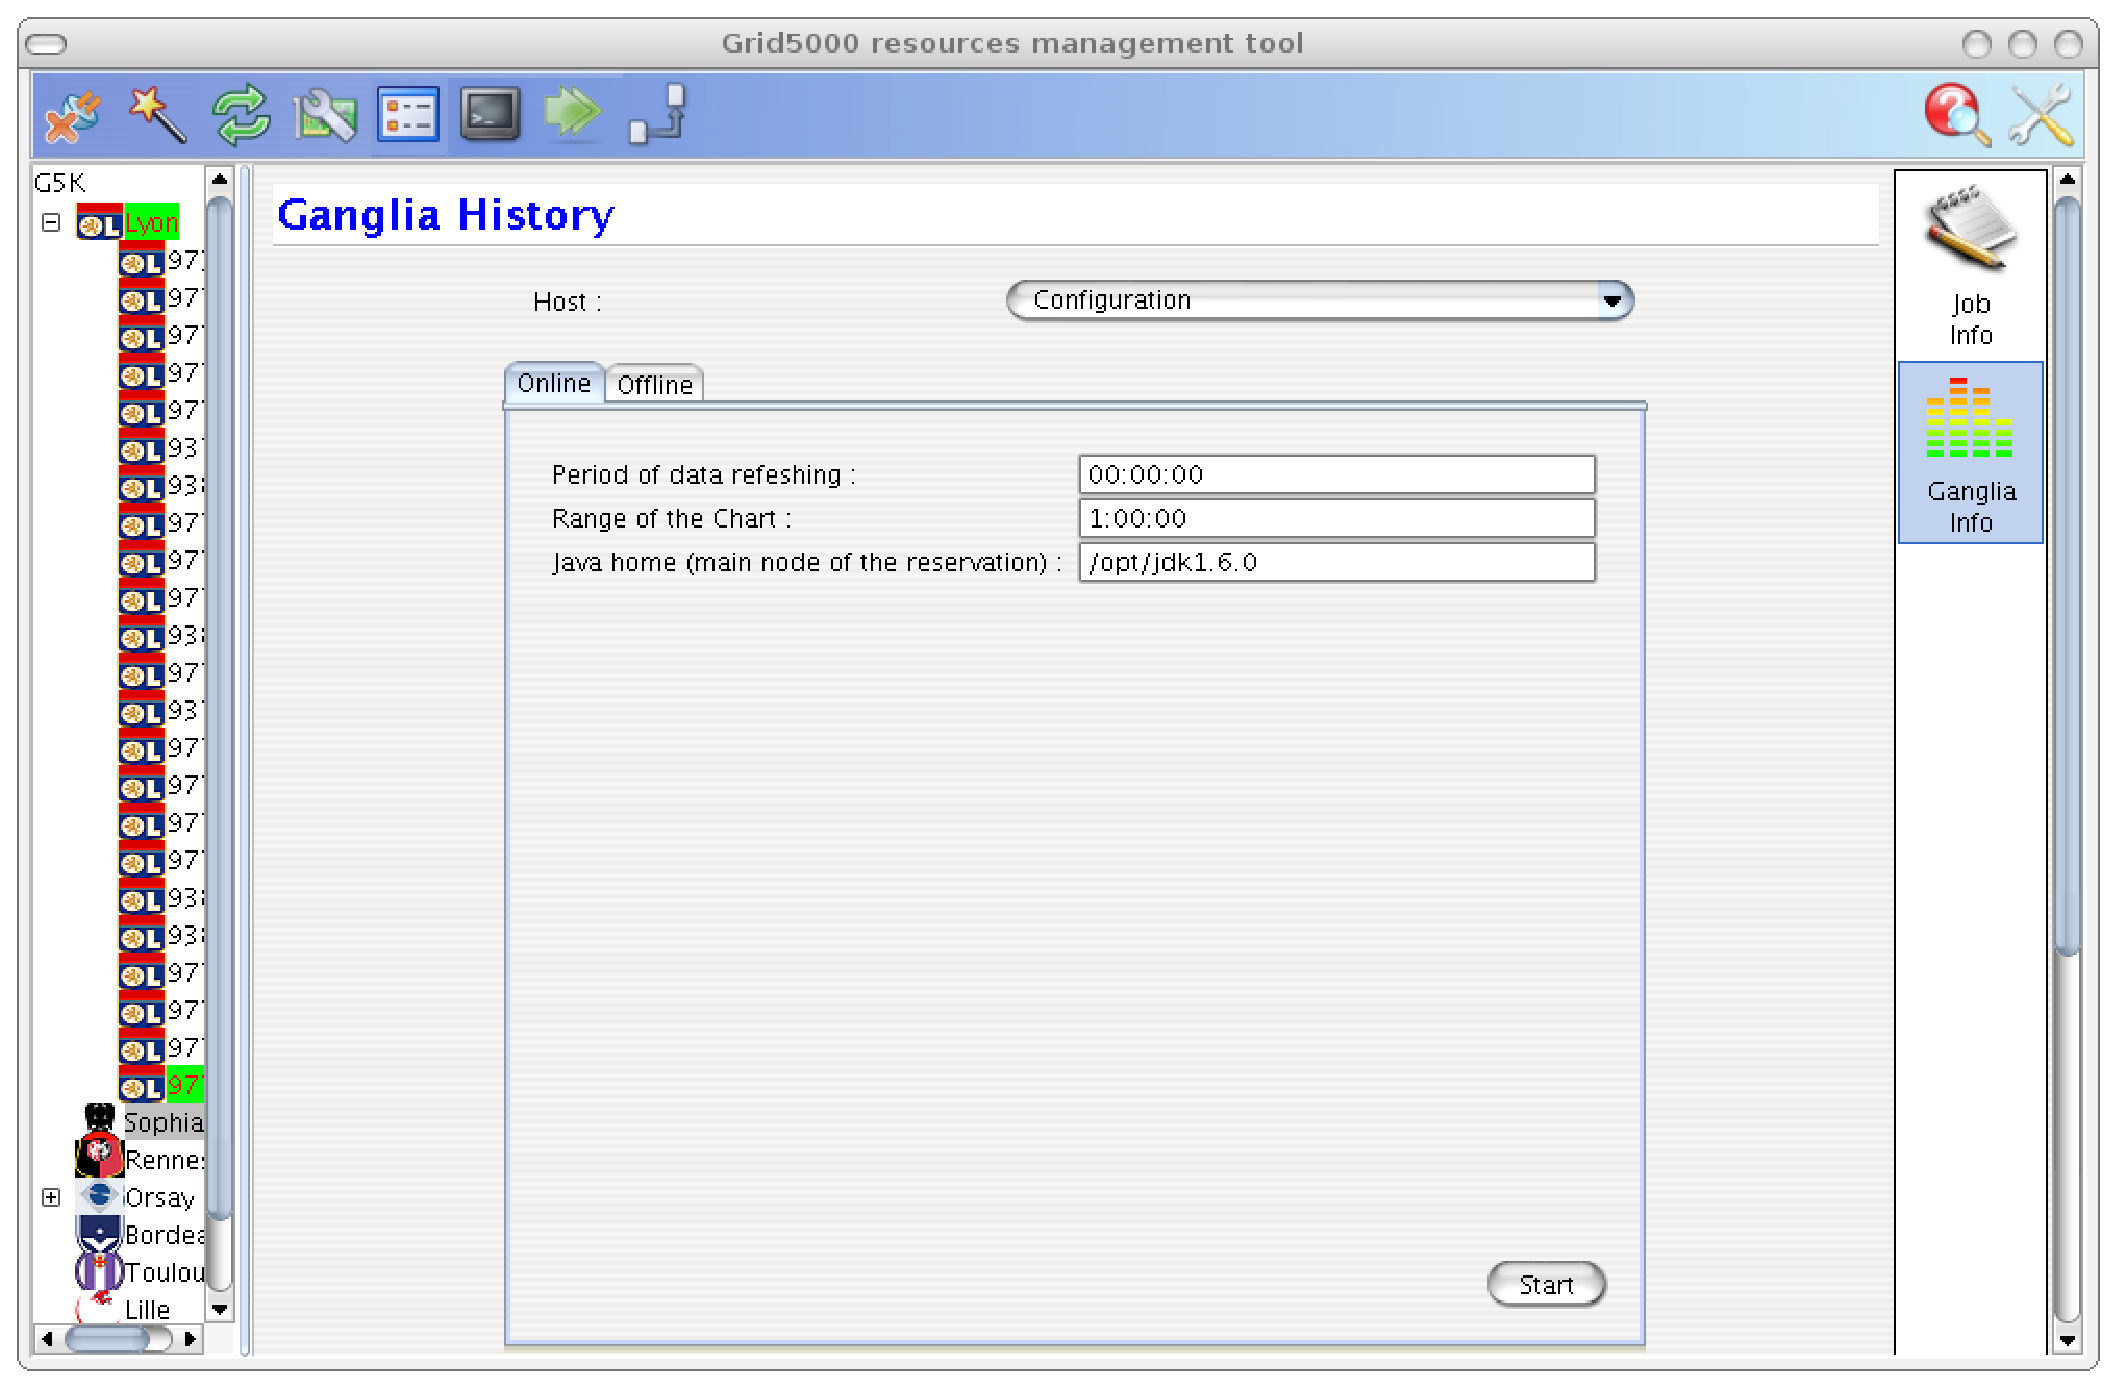
\includegraphics[width=0.5\linewidth]{figures/GRUDU_interface4_ganglia_prerequisites.eps}
  \caption{Configuration of the Ganglia plugin for the job view}
	\label{fig:GRUDU_view_job_ganglia_prerequisites}
  \end{figure}
  \begin{figure}[H]
  \centering
  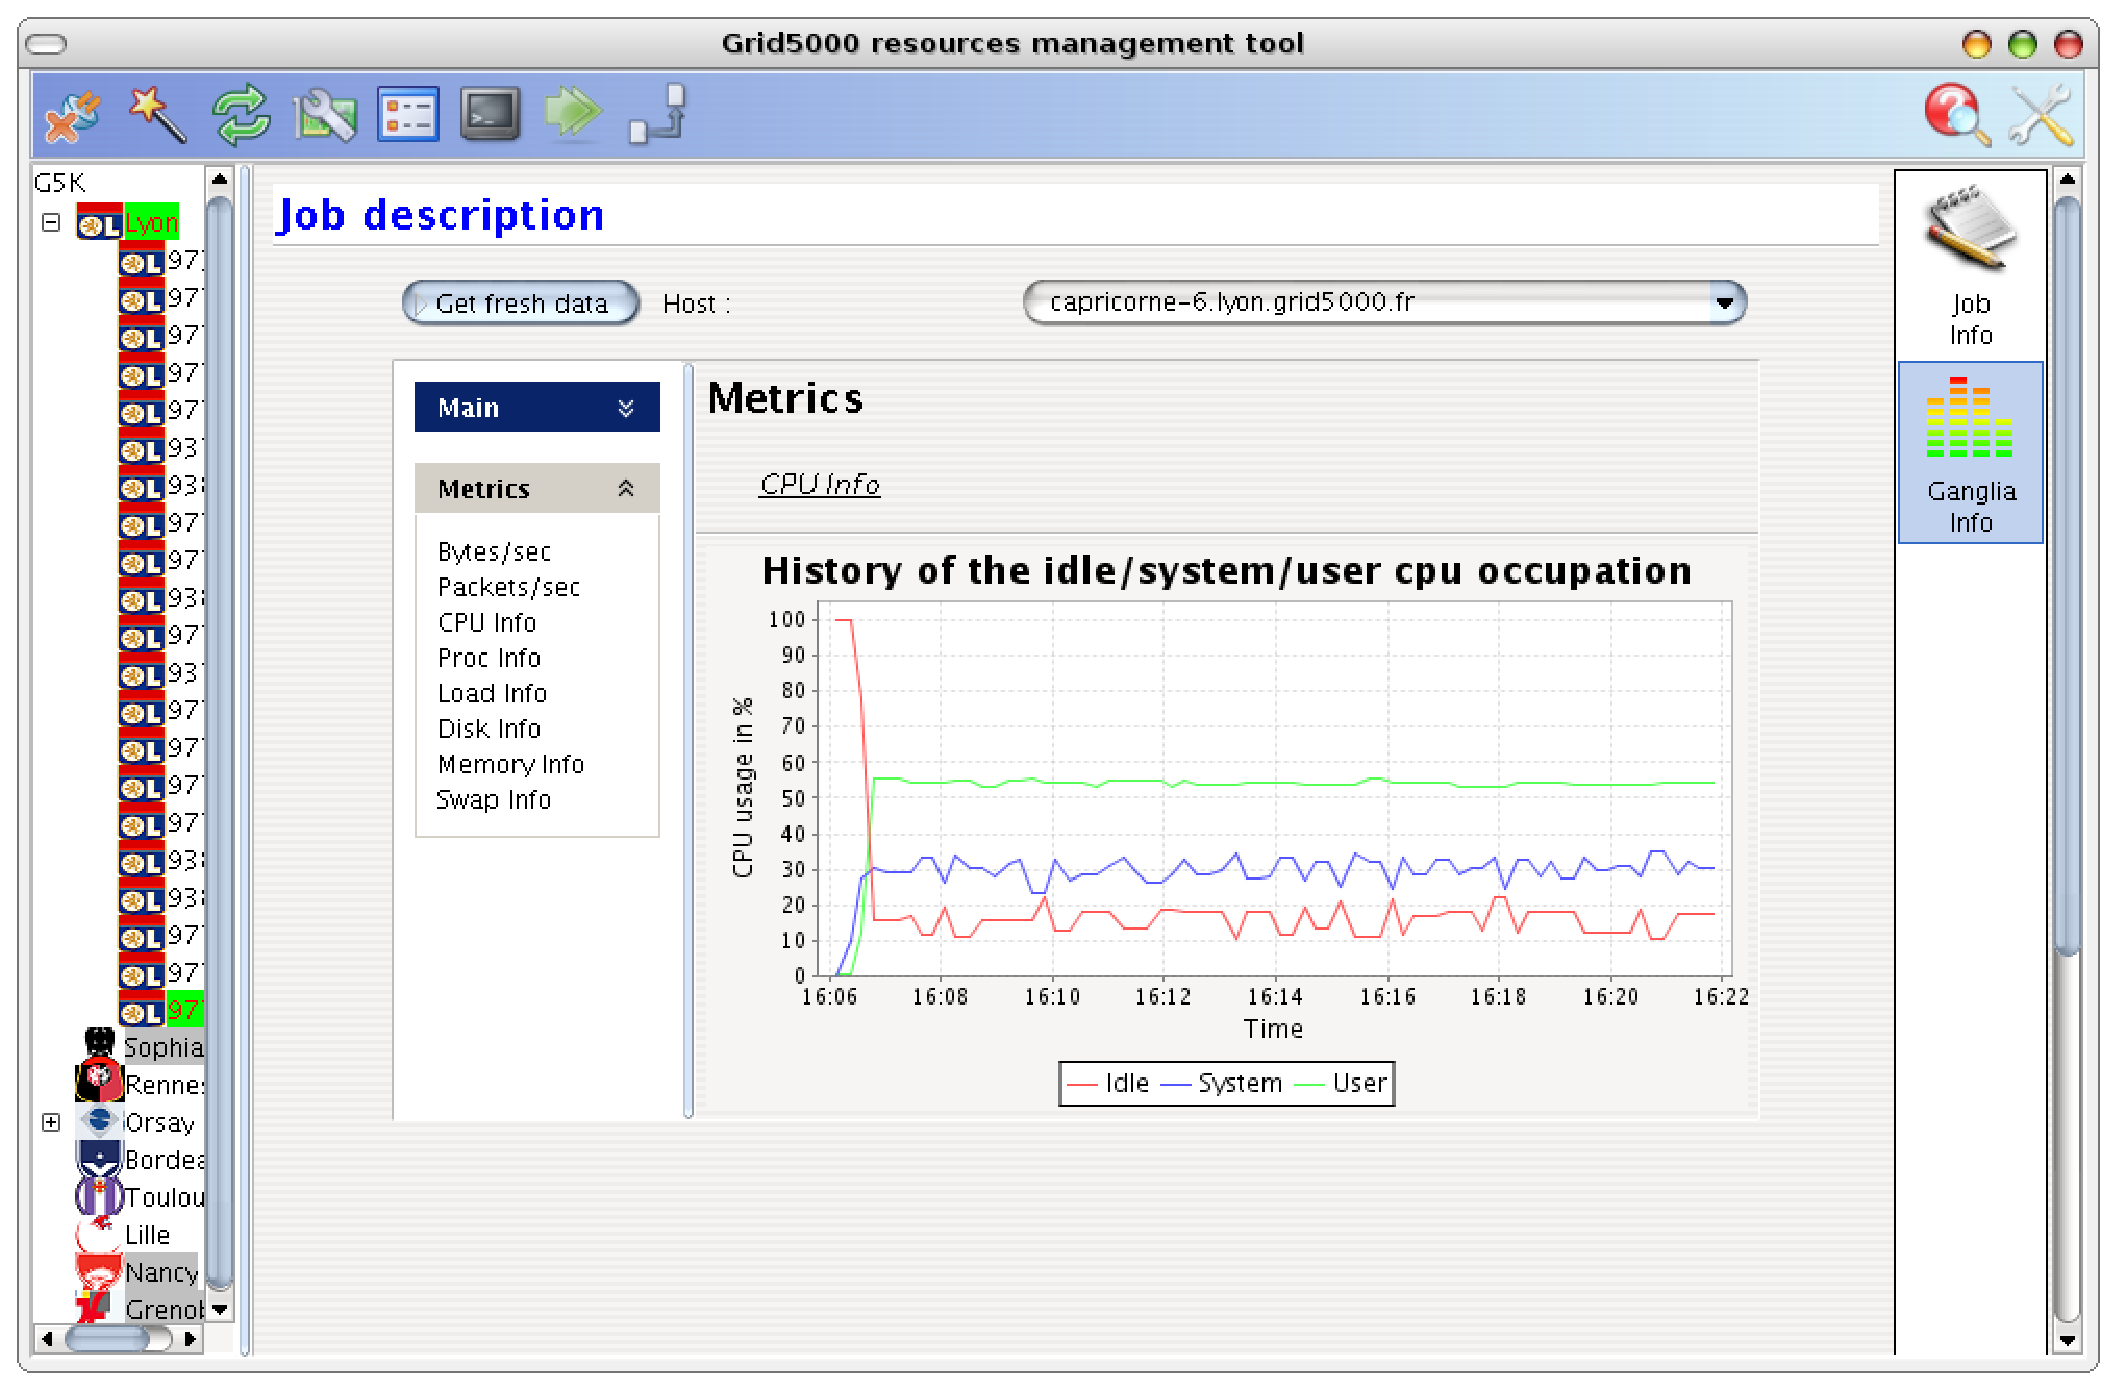
\includegraphics[width=0.5\linewidth]{figures/GRUDU_interface4_ganglia.eps}
  \caption{Ganglia plugin for the job view}
	\label{fig:GRUDU_view_job_ganglia}
  \end{figure}

\end{itemize}



% inclusion de GUM_JFTP.tex
%****************************************************************************%
%* JFTP Module                                                              *%
%*                                                                          *%
%* Author(s):                                                               *%
%* - Abdelkader AMAR (Abdelkader.Amar@ens-lyon.fr)                          *%
%* - David LOUREIRO (David.Loureiro@ens-lyon.fr)                            *%
%*                                                                          *%
%* $LICENSE$                                                                *%
%****************************************************************************%
%* $Id: GUM_JFTP.tex,v 1.5 2007/11/29 16:03:21 dloureir Exp $
%* $Log: GUM_JFTP.tex,v $
%* Revision 1.5  2007/11/29 16:03:21  dloureir
%* typo corrections
%*
%* Revision 1.4  2007/11/29 10:49:23  dloureir
%* Correcting the wrong caption text
%*
%* Revision 1.3  2007/11/08 16:53:48  dloureir
%* Adding the ganglia part in the User's Manual
%*
%* Revision 1.2  2007/11/08 11:31:14  dloureir
%* Correcting the headers
%*
%****************************************************************************%
\chapter{JFTP Module for \grudu}
\section{Presentation}
JFTP is an acronym for \textit{\textbf{J}ava \textbf{F}ile \textbf{T}ransfert
\textbf{P}rotocol}. JFTP is a graphical Java network and file transfer client.
At the origin JFTP is developed as a project under GNU GPL license. You can find
more information about the initial project at
\url{http://j-ftp.sourceforge.net/}. 

JFTP has been modify to corresponds to the needs of the GRUDU users. Thanks to
the modified JFTP you can transfer data between you local machine and \gfk, but
also between \gfk frontales.

\section{Interface}

The JFTP module presents three internal frames, one for the local machine, one
for \gfk with one tab per site, and the last frame for the log of the module.

\begin{figure}[H]
	\centering
	\includegraphics[width=0.7\linewidth]{figures/GRUDU_jftp1.eps}
	\caption{JFTP main interface}
	\label{fig:GRUDU_jftp1}
\end{figure}

For the configuration of the options for the Rsync transfert between \gfk
frontales, you can click on the option menu and you will find the following
frame where you can edit the Rsync options:

\begin{figure}[H]
	\centering
	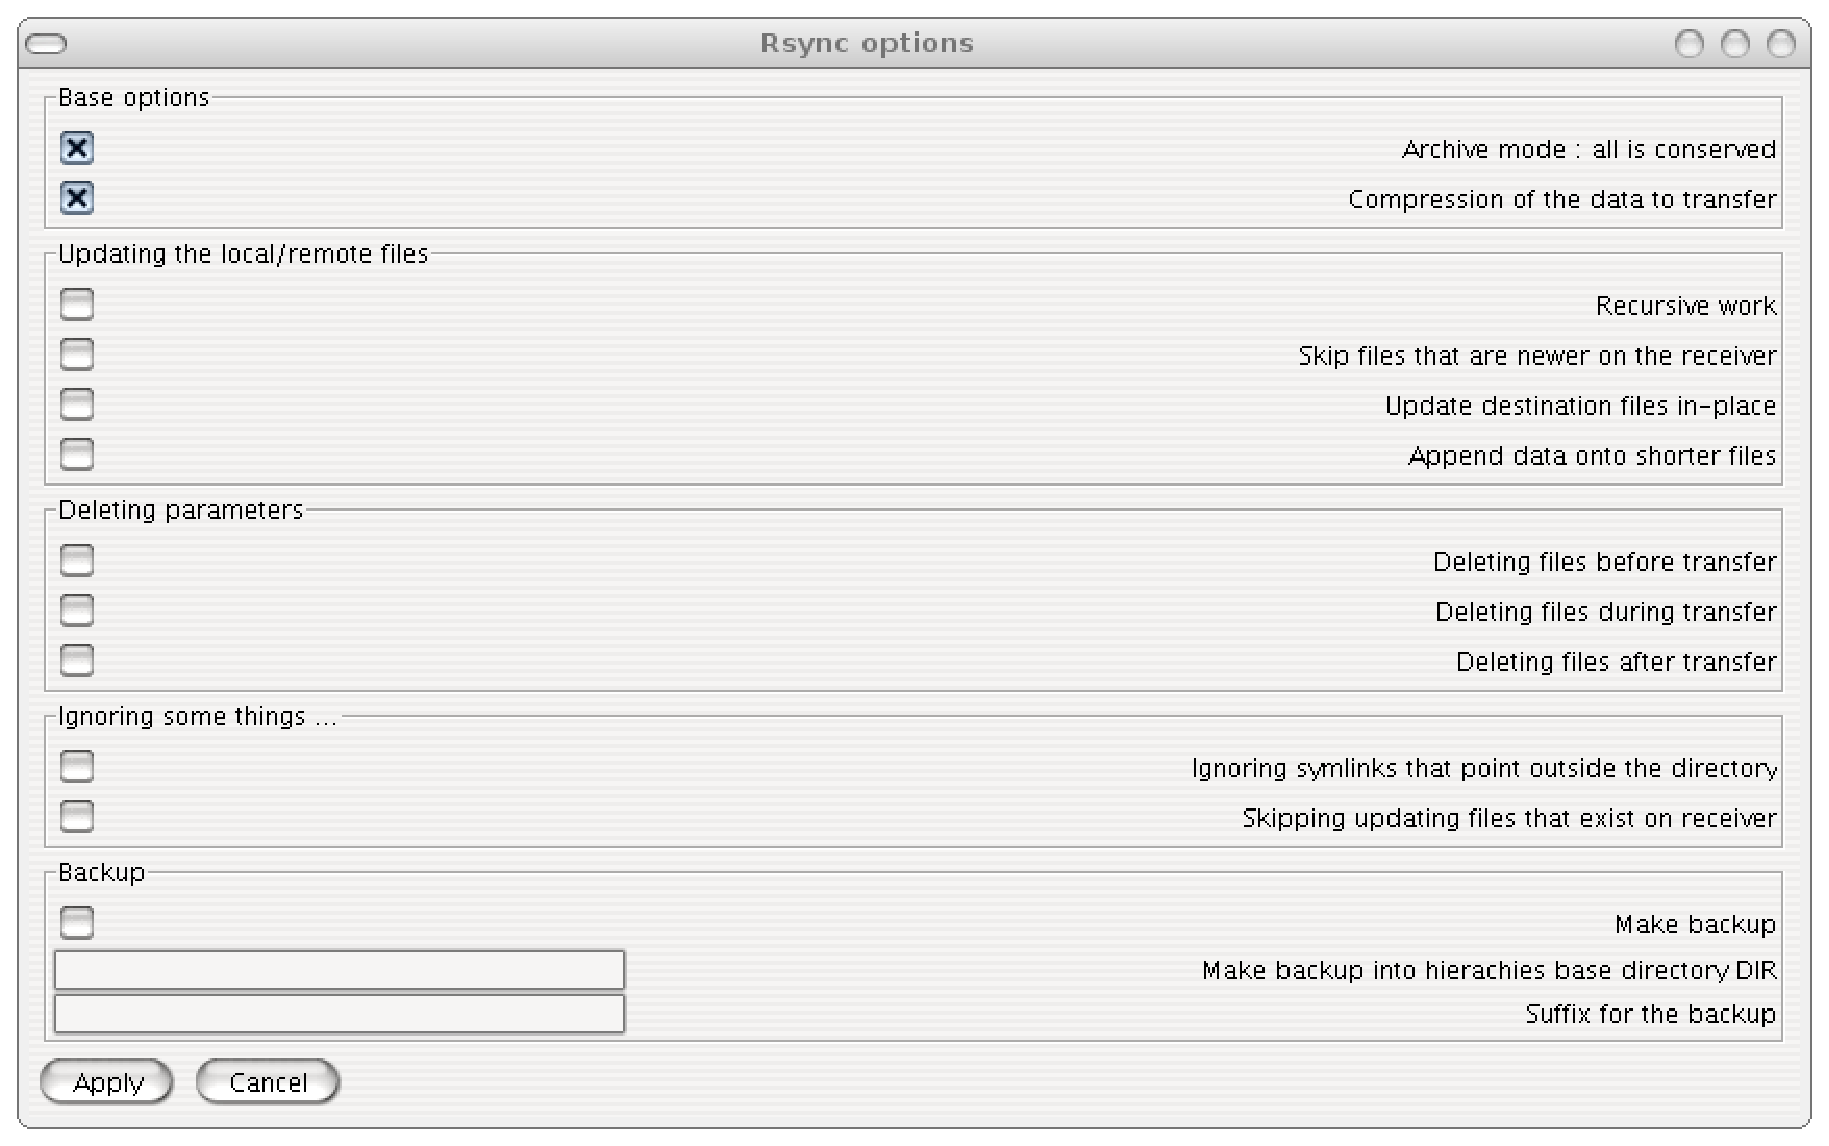
\includegraphics[width=0.5\linewidth]{figures/GRUDU_jftp2.eps}
	\caption{JFTP rsync options}
	\label{fig:GRUDU_jftp2}
\end{figure}

%******************************************%

% inclusion de GUM_Kadeploy.tex
%****************************************************************************%
%* KaDeploy Support                                                         *%
%*                                                                          *%
%* Author(s):                                                               *%
%* - Abdelkader AMAR (Abdelkader.Amar@ens-lyon.fr)                          *%
%* - David LOUREIRO (David.Loureiro@ens-lyon.fr)                            *%
%*                                                                          *%
%* $LICENSE$                                                                *%
%****************************************************************************%
%* $Id: GUM_Kadeploy.tex,v 1.3 2007/11/29 16:03:21 dloureir Exp $
%* $Log: GUM_Kadeploy.tex,v $
%* Revision 1.3  2007/11/29 16:03:21  dloureir
%* typo corrections
%*
%* Revision 1.2  2007/11/08 11:31:14  dloureir
%* Correcting the headers
%*
%****************************************************************************%
\chapter{Deploy your Kadeploy images}
KaDeploy is a fast and scalable deployment system for site and grid
computing. KaDeploy is the reconfiguration system used in \gfk, allowing
the users to deploy their own OS on their reserved nodes.

For more information about how to create and manage KaDeploy images, please
refer to the documentation available on the \gfk web page.

The Figure \ref{fig:GRUDU_kadeploy} shows the frame allowing you to deploy
images on which you have rights. The left hand side of the frame corresponds to
sites and nodes available for deployment (i.e. reserved with the deploy type).
 You can click on the checkboxes to select/deselect the nodes. If you want to 
select/deselect all nodes, you can click on the corresponding button on the 
right-hand side of the frame. Then you can select the image you want to deploy
from the lists on the right hand side of the frame.

When you are done with the configuration, you can click on the deploy
button. A new frame will be displayed corresponding to the log of the deployment
(with both standard output and error).

  \begin{figure}[H]
	\centering
	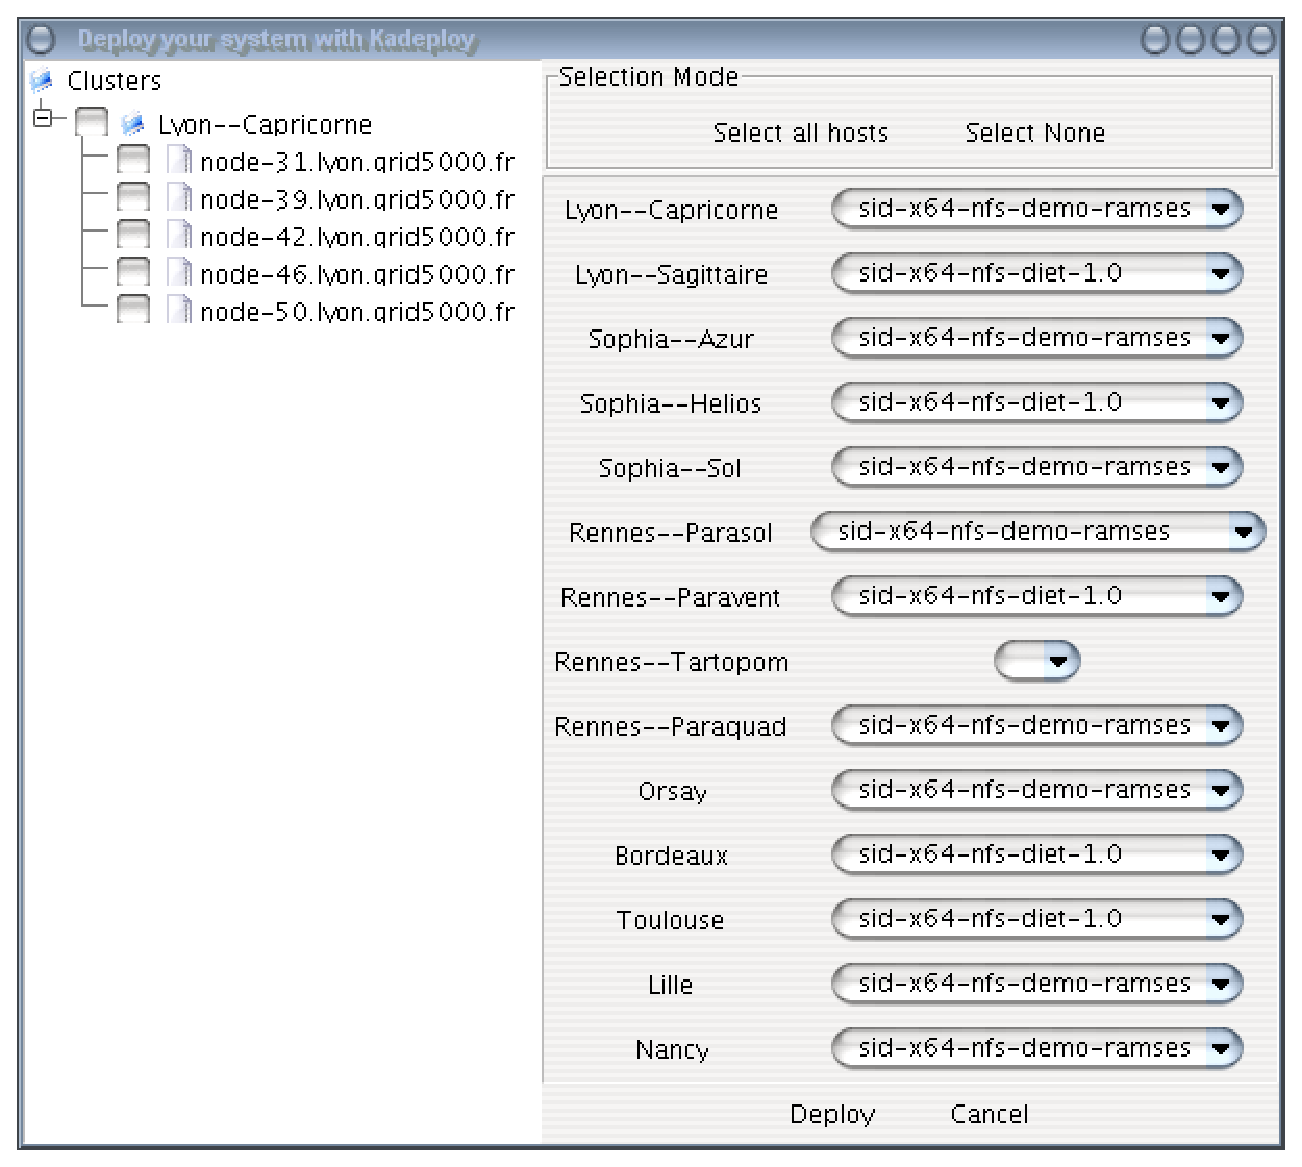
\includegraphics[width=0.5\linewidth]{figures/GRUDU_kadeploy.eps}
	\caption{Kadeploy frame}
	\label{fig:GRUDU_kadeploy}
  \end{figure}

%******************************************%

% inclusion de GUM_applications.tex
%****************************************************************************%
%* Application settings                                                     *%
%*                                                                          *%
%* Author(s):                                                               *%
%* - Abdelkader AMAR (Abdelkader.Amar@ens-lyon.fr)                          *%
%* - David LOUREIRO (David.Loureiro@ens-lyon.fr)                            *%
%*                                                                          *%
%* $LICENSE$                                                                *%
%****************************************************************************%
%* $Id: GUM_applications.tex,v 1.2 2007/11/08 11:31:14 dloureir Exp $
%* $Log: GUM_applications.tex,v $
%* Revision 1.2  2007/11/08 11:31:14  dloureir
%* Correcting the headers
%*
%****************************************************************************%

\chapter{Application settings}
\label{chapter:application_settings}
By clicking the application settings button the following frame appears : 
\begin{figure}[H]
	\centering
	\includegraphics[width=0.6\linewidth]{figures/GRUDU_application_settings.eps}
	\caption{Application settings}
	\label{fig:GRUDU_application_settings}
\end{figure}
For the instance you can only define if you want the tip of the day frame to be
displayed on startup.

%******************************************%

% inclusion de GUI_Troubleshooting.tex
%****************************************************************************%
%* Troubleshooting                                                          *%
%*                                                                          *%
%* Author(s):                                                               *%
%* - Abdelkader AMAR (Abdelkader.Amar@ens-lyon.fr)                          *%
%* - David LOUREIRO (David.Loureiro@ens-lyon.fr)                            *%
%*                                                                          *%
%* $LICENSE$                                                                *%
%****************************************************************************%
%* $Id: GUM_troubleshooting.tex,v 1.3 2007/11/29 16:03:21 dloureir Exp $
%* $Log: GUM_troubleshooting.tex,v $
%* Revision 1.3  2007/11/29 16:03:21  dloureir
%* typo corrections
%*
%* Revision 1.2  2007/11/08 16:28:54  dloureir
%* Adding some corrections and updates
%*
%* Revision 1.1  2007/11/08 11:30:53  dloureir
%* Troubleshooting chapter concerning the possible problems happening during the installation of GRUDU and its use.
%*
%****************************************************************************%

\chapter{Troubleshooting}

Some problems can appear during the installation or during the use of \grudu.
Here are some solutions :
\begin{itemize}
  \item \textbf{\underline{Question :}} \textbf{I am under Gentoo, and when I am launching the
  installer/\grudu, I get the following error :}\\
  \begin{verbatim}
  	java: xcb_xlib.c:50: xcb_xlib_unlock: Assertion `c->xlib.lock' failed.
Aborted
  \end{verbatim}
	\textbf{\underline{Answer : }} This problem come from the Java runtime you are
	using. Simply run the following peace of code in a console and you will be able to run your java application :
	\begin{verbatim}
    CFLAGS="-DNDEBUG" emerge -av1 libxcb
    \end{verbatim}

  \item \textbf{\underline{Question :}} \textbf{I have two screens and when I
  am launching the installer/\grudu, java complains and the following
  exception is raised :}\\
  \begin{verbatim}
Exception in thread "main" java.lang.ExceptionInInitializerError
	at java.lang.Class.forName0(Native Method)
	at java.lang.Class.forName(Class.java:164)
	at java.awt.Toolkit$2.run(Toolkit.java:821)
	at java.security.AccessController.doPrivileged(Native Method)
	at java.awt.Toolkit.getDefaultToolkit(Toolkit.java:804)
	at javax.swing.UIManager.initialize(UIManager.java:1262)
	at javax.swing.UIManager.maybeInitialize(UIManager.java:1245)
	at javax.swing.UIManager.getUI(UIManager.java:851)
	at javax.swing.JPanel.updateUI(JPanel.java:104)
	at javax.swing.JPanel.<init>(JPanel.java:64)
	at javax.swing.JPanel.<init>(JPanel.java:87)
	at javax.swing.JPanel.<init>(JPanel.java:95)
	at diet.application.settings.SettingsPanelImplementation.
<init>(SettingsPanelImplementation.java:13)
	at diet.application.settings.DIETInstallationSettingsPanel.
<init>(DIETInstallationSettingsPanel.java:32)
	at diet.application.DDBApplicationConfiguration.
initializeSpecificSettingsPanelList(DDBApplicationConfiguration.java:49)
	at diet.application.ApplicationConfiguration.
loadConfiguration(ApplicationConfiguration.java:165)
	at diet.application.ApplicationConfiguration.
setApplicationContext(ApplicationConfiguration.java:118)
	at diet.DietOffice.main(DietOffice.java:834)
Caused by: java.lang.ArrayIndexOutOfBoundsException: 1
	at sun.awt.X11GraphicsEnvironment.
getDefaultScreenDevice(X11GraphicsEnvironment.java:178)
	at sun.awt.X11.XToolkit.<clinit>(XToolkit.java:98)
	... 18 more
	\end{verbatim}
\textbf{\underline{Answer : }} To solve this juste launch the installer or
\grudu on the other screen (it should be the first display, under Linux
something like :
\begin{verbatim}
> echo $DISPLAY
:0:0
\end{verbatim}
\end{itemize}

% inclusion de GUM_annexes.tex
%****************************************************************************%
%* Annexes		                                                            *%
%*                                                                          *%
%* Author(s):                                                               *%
%* - Abdelkader AMAR (Abdelkader.Amar@ens-lyon.fr)                          *%
%* - David LOUREIRO (David.Loureiro@ens-lyon.fr)                            *%
%*                                                                          *%
%* $LICENSE$                                                                *%
%****************************************************************************%
%* $Id: GUM_annexes.tex,v 1.3 2007/11/29 16:03:21 dloureir Exp $
%* $Log: GUM_annexes.tex,v $
%* Revision 1.3  2007/11/29 16:03:21  dloureir
%* typo corrections
%*
%* Revision 1.2  2007/11/08 11:31:14  dloureir
%* Correcting the headers
%*
%****************************************************************************%
\appendix
\chapter{Configuration files}

\section{Files used by \grudu}

\grudu uses several configuration files saved in the \texttt{.diet}
directory which is located at the root of your home directory:

\begin{itemize}
  \item \texttt{GRUDUApplicationProperties.xml} : main configuration file containing
  the high level information.
  \item \texttt{g5K.xml} : this file contains the main information for the
  \gfk connection management.
  \item \texttt{g5k\_cfg.xml} : this file corresponds to the grid description.
\end{itemize}

For each file the main content for the \grudu usage will be described.

\section{\gfk configuration file: \textit{GRUDUApplicationProperties.xml}}
\begin{verbatim}
<application>
  <properties 
        name="tipOfTheDayShowOnStartup" 
        value="false" />
  <properties 
        name="tipOfTheDayFileOfTips" 
        value="languages/totd/defaultGRUDUFileOfTips_eng.xml" />
  <properties 
        name="version" 
        value="1.1.0" />
</application>
\end{verbatim}

This files defines the application wide configuration iformation. 

For the moment every elements are a \texttt{properties} with a \texttt{name} and
a \texttt{value}.

For the moment there are three properties declared in that file :
\begin{itemize}
  \item \textit{version} : the purpose of that property is obvious, it
  corresponds to the version of \grudu.
  \item \textit{tipOfTheDayShowOnStartup} : This property declares whether the
  tip of the day should (or not) be displayed on startup.
  \item \textit{tipOfTheDayFileOfTips} : This property defines the file from
  which the tips of the day should be taken.
\end{itemize}

\section{\gfk configuration file: \textit{g5k.xml}}

\begin{verbatim}
<?xml version="1.0" standalone="yes"?>
<g5k>
  <preferredAccesPoint host="acces.lyon.grid5000.fr.fr" />
  <username id="myG5KLogin" />
  <sshkey file="thePathToMySSHKeyFile" />

<!-- G5K Sites -->
 . . .
</g5k>

\end{verbatim}

This file defines the global information used to log in \gfk. The elements that
are not used by \grudu have been removed from the description.

Here are the parameters that should be supplied:

\begin{itemize}
  \item \textit{preferredAccesPoint}: the node has an attribute named
  \textbf{host}. This attribute have to be the name of one of the access
  frontales of \gfk.
  \item \textit{username}: the node has an attribute named \textbf{id} that is
  the login of the user.
  \item \textit{sshkey}: the node has one attribute \textbf{file} which is the
  file storing the ssh private key.
\end{itemize}

\section{\gfk configuration file: \textit{g5k\_cfg.xml}}

\begin{verbatim}

<g5k>
        <site
                 id="Lyon"
                 enable="false"
                 batch_schedulers="OAR1"
         >
                <cluster name="Lyon--Capricorne"  xda="" />
                <cluster name="Lyon--Sagittaire"  xda="" />
        </site>

. . .

</g5k>

\end{verbatim}

This file describes the platform of \gfk, the properties of the sites
(id, batch\_scheduler, etc) but also the clusters of the sites with their
deployment partitions.

Here are the parameters that should be supplied for each site:

\begin{itemize}
  \item \textit{id} : Name of the site
  \item \textit{enable} : (true/false) defines whether the site is considered in
  the interrogation parts of \grudu
  \item \textit{batch\_schedulers} : Name of the batch scheduler to use
  \item For each cluster:
  \begin{itemize}
    \item \textit{name} : the name of the cluster
    \item \textit{xda} : the partition used by KaDeploy
    \end{itemize}
\end{itemize}

%******************************************%

% inclusion de GUM_License.tex
%****************************************************************************%
%* License				                                                    *%
%*                                                                          *%
%* Author(s):                                                               *%
%* - Abdelkader AMAR (Abdelkader.Amar@ens-lyon.fr)                          *%
%* - David LOUREIRO (David.Loureiro@ens-lyon.fr)                            *%
%*                                                                          *%
%* $LICENSE$                                                                *%
%****************************************************************************%
%* $Id: GUM_License.tex,v 1.2 2007/11/08 11:31:14 dloureir Exp $
%* $Log: GUM_License.tex,v $
%* Revision 1.2  2007/11/08 11:31:14  dloureir
%* Correcting the headers
%*
%****************************************************************************%
\chapter{License of GRUDU}
\begin{center}
\begin{scriptsize}
\centering
\verbatiminput{License.txt}
\end{scriptsize}
\end{center}
%******************************************%

\end{document}

% LocalWords:  GRUDU Abdelkader AMAR LOUREIRO IzPack
